% allgem. Dokumentenformat
\documentclass[a4paper,12pt,headsepline]{scrartcl}
%Variablen welche innerhalb der gesamten Arbeit zur Verfügung stehen sollen
\newcommand{\titleDocument}{Studienarbeit ``Entwicklung einer Running-App f\H{u}r Android''}
\newcommand{\subjectDocument}{im Studiengang ``International Applied Computer Science''}

% Subsubsubsection
\setcounter{tocdepth}{5}

% weitere Pakete
% Grafiken aus PNG Dateien einbinden
\usepackage{graphicx}

% Deutsche Sonderzeichen benutzen 
\usepackage{ngerman}

% deutsche Silbentrennung
\usepackage[ngerman]{babel}

% Eurozeichen einbinden
\usepackage[right]{eurosym}

% Umlaute unter UTF8 nutzen
\usepackage[utf8]{inputenc}

% Zeichenencoding
\usepackage[T1]{fontenc}

\usepackage{lmodern}
\usepackage{fix-cm}

% floatende Bilder ermöglichen
%\usepackage{floatflt}

% mehrseitige Tabellen ermöglichen
\usepackage{longtable}

% Unterstützung für Schriftarten
%\newcommand{\changefont}[3]{ 
%\fontfamily{#1} \fontseries{#2} \fontshape{#3} \selectfont}

% Packet für Seitenrandabständex und Einstellung für Seitenränder
\usepackage{geometry}
\geometry{left=3.5cm, right=3cm, top=3cm, bottom=3cm}

% Paket für Boxen im Text
\usepackage{fancybox}

% bricht lange URLs "schoen" um
\usepackage[hyphens,obeyspaces,spaces]{url}

% Paket für Textfarben
\usepackage{color}

% Mathematische Symbole importieren
\usepackage{amssymb}

% auf jeder Seite eine Überschrift (alt, zentriert)
%\pagestyle{headings}

% erzeugt Inhaltsverzeichnis mit Querverweisen zu den Kapiteln (PDF Version)
\usepackage[bookmarksnumbered,pdftitle={\titleDocument},hyperfootnotes=false]{hyperref} 
%\hypersetup{colorlinks, citecolor=red, linkcolor=blue, urlcolor=black}
%\hypersetup{colorlinks, citecolor=black, linkcolor= black, urlcolor=black}

% neue Kopfzeilen mit fancypaket
\usepackage{fancyhdr} %Paket laden
\pagestyle{fancy} %eigener Seitenstil
\fancyhf{} %alle Kopf- und Fußzeilenfelder bereinigen
\fancyhead[L]{\nouppercase{\leftmark}} %Kopfzeile links
\fancyhead[C]{} %zentrierte Kopfzeile
\fancyhead[R]{\thepage} %Kopfzeile rechts
\renewcommand{\headrulewidth}{0.4pt} %obere Trennlinie
%\fancyfoot[C]{\thepage} %Seitennummer
%\renewcommand{\footrulewidth}{0.4pt} %untere Trennlinie

% für Tabellen
\usepackage{array}

% Runde Klammern für Zitate
%\usepackage[numbers,round]{natbib}

% Festlegung Art der Zitierung - Havardmethode: Abkuerzung Autor + Jahr
\bibliographystyle{alphadin}

% Schaltet den zusätzlichen Zwischenraum ab, den LaTeX normalerweise nach einem Satzzeichen einfügt.
\frenchspacing

% Paket für Zeilenabstand
\usepackage{setspace}

% für Bildbezeichner
\usepackage{capt-of}

% für Stichwortverzeichnis
\usepackage{makeidx}

% für Listings
\usepackage{listings}
\lstset{numbers=left, numberstyle=\tiny, numbersep=5pt, keywordstyle=\color{black}\bfseries, stringstyle=\ttfamily,showstringspaces=false,basicstyle=\footnotesize,captionpos=b}
\lstset{language=java}

% Indexerstellung
\makeindex

% Abkürzungsverzeichnis
\usepackage[german]{nomencl}
\let\abbrev\nomenclature

% Abkürzungsverzeichnis LiveTex Version
\renewcommand{\nomname}{Abkürzungsverzeichnis}
\setlength{\nomlabelwidth}{.25\hsize}
\renewcommand{\nomlabel}[1]{#1 \dotfill}
\setlength{\nomitemsep}{-\parsep}
\makenomenclature
%\makeglossary

% Abkürzungsverzeichnis TeTEX Version
% \usepackage[german]{nomencl}
% \makenomenclature
% %\makeglossary
% \renewcommand{\nomname}{Abkürzungsverzeichnis}
% \setlength{\nomlabelwidth}{.25\hsize}
% \renewcommand{\nomlabel}[1]{#1 \dotfill}
% \setlength{\nomitemsep}{-\parsep}

% Disable single lines at the start of a paragraph (Schusterjungen)
\clubpenalty = 10000
% Disable single lines at the end of a paragraph (Hurenkinder)
\widowpenalty = 10000
\displaywidowpenalty = 10000

\begin{document}
% hier werden die Trennvorschläge inkludiert
%hier müssen alle Wörter rein, welche Latex von sich auch nicht korrekt trennt bzw. bei denen man die genaue Trennung vorgeben möchte
\hyphenation{
Film-pro-du-zen-ten
Lux-em-burg
Soft-ware-bau-steins
zeit-in-ten-siv
}

%Schriftart Helvetica
%\changefont{phv}{m}{n}

% Titelseite %
% das Papierformat zuerst
%\documentclass[a4paper, 11pt]{article}

% deutsche Silbentrennung
%\usepackage[ngerman]{babel}

% wegen deutschen Umlauten
%\usepackage[ansinew]{inputenc}

% hier beginnt das Dokument
%\begin{document}


\thispagestyle{empty}

%\begin{figure}[t]
% \includegraphics[width=0.6\textwidth]{abb/fh_koeln_logo}
%\end{figure}

\begin{figure}[t]
 \centering
 
\includegraphics[width=0.15\textwidth]{abb/app_icon}
%~~~~~~~~~~
 
\includegraphics[width=0.3\textwidth]{abb/dhbw_logo}
\end{figure}


\begin{verbatim}


\end{verbatim}

\begin{center}
\Large{Duale Hochschule Baden-Württemberg}\\
\Large{- Standort Stuttgart -}\\
\end{center}


\begin{center}
\Large{Fakultät für Technik}
\end{center}
\begin{verbatim}




\end{verbatim}
\begin{center}
\doublespacing
\textbf{\LARGE{\titleDocument}}\\
\singlespacing
\begin{verbatim}

\end{verbatim}
\textbf{{\subjectDocument}}
\end{center}
\begin{verbatim}

\end{verbatim}
\begin{center}

\end{center}
\begin{verbatim}

\end{verbatim}
\begin{verbatim}






\end{verbatim}
\begin{flushleft}
\begin{tabular}{llll}
\textbf{Thema:} & & Entwicklung einer Running-App für Android & \\
& & \\
\textbf{Autoren:} & & Roland Weinreich& \\
& & roland.weinreich@gmail.com & \\
& & MatNr. 5885985 & \\
& & \\
& & Franz Flintzer& \\
& & fflintzer@gmail.com & \\
& & MatNr. 8677472 & \\
& & \\
\textbf{Version vom:} & & \today &\\
& & \\
\textbf{Betreuer:} & & Prof. Dr. Karl Friedrich Gebhardt &\\
\end{tabular}
\end{flushleft}

% römische Numerierung
%\pagenumbering{arabic}

% 1.5 facher Zeilenabstand
\onehalfspacing

% Sperrvermerk
%\section*{Sperrvermerk}
\textcolor{red}{
Die vorliegende Arbeit beinhaltet interne und vertrauliche Informationen der Firma <Firmenname>.
Die Weitergabe des Inhalts der Arbeit im Gesamten oder in Teilen sowie das Anfertigen
von Kopien oder Abschriften - auch in digitaler Form - sind grundsätzlich untersagt.
Ausnahmen bedürfen der schriftlichen Genehmigung der Firma <Firmenname>.
}

% Einleitung / Abstract
\section*{Zusammenfassung}


%\begin{verbatim}

%

%\end{verbatim}

\section*{Abstract}


% einfacher Zeilenabstand
\singlespacing

% Inhaltsverzeichnis anzeigen
\newpage
\tableofcontents

% das Abbildungsverzeichnis
%\newpage
% Abbildungsverzeichnis soll im Inhaltsverzeichnis auftauchen
\addcontentsline{toc}{section}{Abbildungsverzeichnis}
% Abbildungsverzeichnis endgueltig anzeigen
\listoffigures

% das Tabellenverzeichnis
%\newpage
% Abbildungsverzeichnis soll im Inhaltsverzeichnis auftauchen
\addcontentsline{toc}{section}{Tabellenverzeichnis}
% \fancyhead[L]{Abbildungsverzeichnis / Abkürzungsverzeichnis} %Kopfzeile links
% Abbildungsverzeichnis endgueltig anzeigen
\listoftables

%% WORKAROUND für Listings
%\makeatletter% --> De-TeX-FAQ
%\renewcommand*{\lstlistoflistings}{%
%  \begingroup
%    \if@twocolumn
%      \@restonecoltrue\onecolumn
%    \else
%      \@restonecolfalse
%    \fi
%    \lol@heading
%    \setlength{\parskip}{\z@}%
%    \setlength{\parindent}{\z@}%
%    \setlength{\parfillskip}{\z@ \@plus 1fil}%
%    \@starttoc{lol}%
%    \if@restonecol\twocolumn\fi
%  \endgroup
%}
%\makeatother% --> \makeatletter
% das Listingverzeichnis
%\newpage
% Listingverzeichnis soll im Inhaltsverzeichnis auftauchen
\addcontentsline{toc}{section}{Listingverzeichnis}
\fancyhead[L]{Abbildungs- / Tabellen- / Listingverzeichnis} %Kopfzeile links
\renewcommand{\lstlistlistingname}{Listingverzeichnis}
\lstlistoflistings
%%%%

% das Abkürzungsverzeichnis
%\newpage
% Abkürzungsverzeichnis soll im Inhaltsverzeichnis auftauchen
\addcontentsline{toc}{section}{Abkürzungsverzeichnis}
% das Abkürzungsverzeichnis entgültige Ausgeben
\fancyhead[L]{Abkürzungsverzeichnis} %Kopfzeile links
\nomenclature{API}{Application Programming Interface}
\nomenclature{DHBW}{Duale Hochschule Baden Württemberg}
\nomenclature{AOSP}{Android Open Source Project}
\nomenclature{GPX}{GPS Exchange Format}
\nomenclature{GPS}{Global Positioning System}
\nomenclature{UI}{User Interface}
\printnomenclature

% Definiert Stegbreite bei zweispaltigem Layout
\setlength{\columnsep}{25pt}

%%%%%%% EINLEITUNG %%%%%%%%%%%%
%\twocolumn
\newpage
\fancyhead[L]{\nouppercase{\leftmark}} %Kopfzeile links

% 1,5 facher Zeilenabstand
\onehalfspacing

% einzelne Kapitel
\section{Einleitung}\label{einleitung}
Als duale Studenten an unterschiedlichen Praxis- und Theoriestandorten gibt es längere Zeiträume in denen man Familie und Freunde nicht sehen kann. Das gemeinsame Joggen in der Freizeit fällt dann natürlich auch weg. Dazu kommen verschiedene Arbeitszeiten und teils sogar verschiedene Zeitzonen, die ein Treffen schon zeitlich nicht zulassen würden. 

Besonders fehlen dann die Motivation überhaupt Sport zu machen sowie der gegenseite Ansporn durchzuhalten oder das Tempo zu steigern. 

Genau hier möchten wir mit unserer Android-App ansetzen, die es Läufern erlaubt, zeitlich und vom Ort unabhänigig gegeneinander anzutreten.

\section{Architektur}\label{kapitel2}
\subsection{Überblick}
\begin {figure}[htb]
\centering
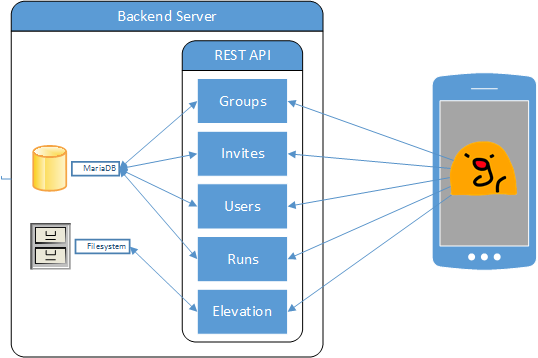
\includegraphics{abb/network_diagram_visio}
\caption{Kommunikation zwischen App und Backend-Server}
\end{figure}
Im folgenden erkläre ich die auf der Abbildung dargestellten Komponenten und warum diese für das Projekt gewählt wurden.
\subsection{Backend Server}
\subsubsection{Betriebssystem}
Bei dem Betriebssystem auf dem Backendserver handelt es sich um die Linux-Distribution Ubuntu der Version 14.04.2. Diese eignet sich besonders gut für den Einsatz auf einem möglichst dauerhaft erreichbaren Server da es sich um ein Long-Term-Support-Version handelt. Diese garantiert die Versorgung mit Sicherheits- und Wartungs-Updates für fünf Jahre ab Veröffentlichung.
\subsubsection{Datenbank}
Als Datenbankverwaltungssystem  haben wir uns entschieden ``MariaDB'' zu nutzen. MariaDB ist das Pendant zu ``MySQL'', jedoch ist es schneller, sicherer und hat eine aktivere Community.
Beide Teammitglieder könne bereits auf längere Erfahrung in MySQL zurückgreifen. Die Arbeit mit MariaDB war aufgrund des weitgehend identischen Befehlssatzes sehr unkompliziert. %HIBERNATE!
\subsubsection{REST API}
Um der App eine geeignete Schnittstelle zu Daten über das Internet bereitzustellen haben wir uns für eine REST API entschieden.
REST steht für ``Representational State Transfer'', einem stetig wachsenden Architekturmodell für Client-Server-Kommunikation bei Web Services.
\paragraph{REST Allgemein}
REST ist zustandslos, d.h. jede Nachricht enthält genügend Informationen um den Inhalt zu verstehen. Das ist besonders wichtig mit Augenmerk auf Skalierbarkeit. So ist die Lastenverteilung der REST-Anfragen auf mehrere Systeme sehr einfach, da keine sitzungspezifischen Daten o.Ä. zwischen den Servern synchronisiert werden müssen. Das gleiche gilt natürlich auch für High-Availability-Systeme.

REST schöpft den HTTP Funktionsumfang weitgehend aus, um u.A. erweitertes Caching und eine hohe Selbsterklärungsfähigkeit zu garantieren.

So erlaubt die Operation ``POST'' es, neue Ressourcen zu erstellen.

``GET'' ermöglicht es, Resourcen anzufragen. ``GET'' ist nullipotent, d.h. es werden unter Garantie keine Änderungen an der Ressource stattfinden.

Mit ``PUT'' kann man eine Ressource ersetzen, mit ``DELETE'' löschen. Diese beiden Operationen bezeichnet man als ``idempotent''. Das bedeutet dass die Anfrage das gleiche Ergebnis produzieren wird, egal wie häufig diese wiederholt wird.

Jeder Ressource ist genau eine URL zugeordnet. Beispielsweise bekommt so der Client mit einer Anfrage mit der Operation ``GET'' auf ``myserver.com/run'' die Liste aller Läufe zurück, während die gleiche Anfrage auf ``myserver.com/run/15'' nur den Lauf mit der ID 15 zurückgibt. 

Ein weitere Eigenschaft von REST ist es, dass die Kommunikationsform nicht standardisiert ist. So ist es möglich, anhand von Daten verpackt in JSON, HTML, XML oder auch in einem komplett eigenen Format zu kommunizieren.
\paragraph{Spring Framework und Tomcat}
Für die Realisierung der Webservices haben wir uns entschieden das Spring Framework zu nutzen.
Ersteres wurde gewählt da es bei einem Teammitglied relevant für die Bachelorarbeit wird und sich so in das Framework eingearbeitet werden konnte. 

Das quelloffene Framework erlaubt es u.A. skalierbare, performante, reichhaltige Web-Services aufzusetzen. Es ist möglich spezifische Sicherheitsmaßnahmen umzusetzen, JSON, XML o.Ä. automatisch zu serialisieren und deserialisieren, Anfragen zu validieren usw., d.h. es ist mehr als ausreichend für den Rahmen dieser Studienarbeit.

Die Programmierung im Spring-Framework erfolgt mit Java (mit zusätzlichen Annotationen) und XML. Es vereinfacht das Programmierprinzip Dependency Injection durch wahlweise das automatische Einlesen von hinterlegten XML-Dateien oder Annotationen im Java-Code. Auch das Programmierparadigma ``Aspektorientierte Programmierung'' wird dem Programmierer nahegelegt.
Spring besteht aus vielen kleineren Frameworks, von denen einige Verwendung im Projekt gefunden haben:
\begin{itemize}
\item Sping Core - Das ``Kern''-Framework.
\item Spring Web - Um Web-Applikationen zu erstellen.
\item Spring Web MVC - Fügt ein DispatcherServlet hinzu dass Anfragen an Handler/Controller weiterleitet und damit das MVC-Programmiermuster stark vereinfacht.\footnote{Introduction to Spring Web MVC framework, vgl.~\cite{webmvc}~[S.437]}. 
\item Spring Security - Die Sicherheitskomponente für das Spring Framework.
\end{itemize}

Als Application Server wurde Tomcat gewählt, da beide Teammitglieder diesen vorher bereits mehrfach aufsetzen durften und eventuell spätere Sicherheitsmaßnahmen wie das Einbinden eines Zertifikats um den HTTP-Verkehr über SSL zu verschlüsseln in wenigen Minuten möglich ist.
\paragraph{JSON}
Als Format für den Austausch von Daten zwischen Server und Client haben wir uns für JSON entschieden.

JSON weist im Vergleich zum stärksten Konkurrenten XML eine hohe Lesbarkeit auf und lässt sich sowohl auf dem Server als auch auf der App sehr einfach von und zu Java-Objekten serialisieren und deserialisieren.

Auf dem Server übernimmt diese Aufgabe Jackson, auf der App Gson.
\paragraph{Maven}
Das manuelle Einbinden von JARs in Java-Projekte stellt eine Herausforderung da. Hierbei müssen diese von vertrauenswürdigen Quellen manuell heruntergeladen werden, in den richtigen Ordner verschoben und importiert werden.

Um den Aufwand zu minimieren nutzen wir Maven, welche sich selbst um das Herunterladen und Einbinden der Java-Archive kümmert. Dabei ist auch das Aktualisieren der Pakete durch das Ändern einer einzigen Zeile in der Maven-Konfigurationsdatei möglich.
\subsection{App}
Die App ist für Android 5.0 ab API 21 geschrieben. 

Für das Betriebssystem Android haben wir uns entschieden da beide Teammitglieder ein Android-Smartphone besitzen. Da es sich bei dieser Studienarbeit um kein Projekt mit wirtschaftlicher Motivation handelt und die API einige Verbesserungen gegenüber älteren Versionen mitbringt hielt uns von der Entscheidung auch nicht die relativ geringe Verbreitung von 12,4\% der APIs 21 und 22 ab\footnote{Dashboards, vgl.~\cite{verbreitung}} (Stand 1. Juni 2015).

\section{Analyse}\label{kapitel4}
\subsection{Einleitung}
\subsubsection{Zweck der Anwendung}
Die App soll es ermöglichen, einen Lauf mitzuschneiden, um ihn anschließend an eine Gruppe von Freunden zu veröffentlichen. Diesen ist es dann möglich, mit ihren Freunden zu laufen bzw. gegen diese anzutreten. Läufe sollen regelmäßig (z.B. einmal pro Woche) stattfinden, um ein regelmäßiges zurückkehren zu unserer App und dem Sport zu gewährleisten. Um Läufe vergleichbar zu machen sollen Höhendaten berücksichtigt werden, um Läufern auf bergigen Strecken, die anstrengender zu Laufen sind eine faire Chance zu geben.

Während des Laufes soll ein direkter Vergleich zur Konkurrenz möglich sein. Dies geschieht durch die Einblendung sogenannter Geister, also die Darstellung des Fortschritts der bereits gelaufenen Gegner im Vergleich zum eigenen. Auch während des Laufens werden Nutzer so angetrieben, ihr Bestes zu geben.

Um die Funktionalität zu gewährleisten sind das Schreiben einer Android-App und das Aufzetzen eines Webserver nötig, der als zentraler Datenspeicher agiert und die verschiedenen Nutzer verbindet.
\subsubsection{Projektumfang}
Ziel der App ist es nicht, wie andere Fitness-, bzw. Joggingapps umfangreiche Statistiken anzubieten. Vielmehr konzentrieren wir uns in der Arbeit darauf, Gamification zu nutzen und durch den direkt ersichtlichen Wettbewerb die Nutzer anzuspornen. Statt ausführlicher Statistiken soll ein GPX-Export ermöglicht werden, damit Nutzer ihre Läufe später in beliebiger Software importieren und auswerten können. So ist unsere App keine Konkurrenz zu vielen etablierten Fitnessportalen, sondern lässt sich als Ergänzung nutzen.

Weiterhin ist es keine Anforderung, ein vollständiges Social Network mit Privat- und Gruppenunterhaltungen bereitzustellen. Diese Funktionalität kann in späteren Versionen der App durchaus implementiert werden, ist aber nicht Hauptaspekt der Studienarbeit. Wichtig ist dagegen, Funktionalität anzubieten um Gruppen zu verwalten, also Nutzer hinzuzufügen und zu löschen.

Die Benutzeroberfläche der App soll ansprechend gestaltet werden, dennoch ist sie nicht Hauptaspekt der Arbeit, da dies in Kombination mit der übrigen Funktionalität den Rahmen einer Studienarbeit sprengen würde. Insbesondere der Bildschirm während des Laufens soll hierbei ein Wiedererkennungsmerkmal darstellen. In der Version, die während der Studienarbeit geschrieben wird, soll ersichtlich werden, wie eine spätere, professionell gestaltete Oberfläche aussehen könnte.

Wir können keinen direkten Einfluss auf die Skalierbarkeit und Verfügbarkeit des Webservers nehmen, da dieser auf einer virtuellen Maschine der DHBW läuft. Dennoch sollte der Webserver aus programmatischer Sicht gewissen Performanceanforderungen genügen.
\subsection{Funktionale Anforderungen}
\subsubsection{Webserver}
Der Webserver stellt dem Klienten eine Schnittstelle bereit, um Nutzer, Gruppen und Läufe zu verwalten. Er muss dabei folgende Funktionale Anforderungen erfüllen:
\begin{itemize}
\item Authentifizierung durch Nutzername und Passwort
\item Erstellen und Herausgeben eines Authentifizierungstokens bei Erfolg
\item Authentifizierung durch das Authentifizierungstoken, Zuordnung zum jeweiligen Nutzer
\item Erstellen und Löschen von Nutzern
\item Ausgabe und Modifikation von Nutzerdaten
\item Erstellen und Löschen von Gruppen
\item Ausgabe und Modifikation von Gruppendaten
\item Hinzufügen und Entfernen von Nutzern zu Gruppen
\item Unterscheidung von Gruppenadministratoren und Nutzern
\item Einladen von Nutzern in Gruppen
\item Annehmen und Ablehnen von Einladungen
\item Verwaltung regelmäßiger Stichtage zur Laufauswertung
\item Erstellen und Ausgeben von Läufen, abhängig von Nutzer und Gruppe
\item Ausgabe von Kacheln mit Höhendaten
\end{itemize}
\subsubsection{Android App}
Die Android App muss folgende Funktionalität erfüllen:
\begin{itemize}
\item Anmeldung beim Webserver mit Nutzername und Passwort
\item Speicherung von Anmeldedaten
\item Speicherung des Authentifizierungstokens
\item Authentifizierung beim Webserver mit Authentifizierungstoken
\item Registrierung beim Webserver
\item Abmeldung inklusive Entfernung von Token und Anmeldedaten
\item Anzeigen einer Übersichte aller Gruppen
\item Erstellen von neuen Gruppen
\item Anzeigen einer Übersicht aller Nutzer und aktuellen Läufe einer Gruppe, inklusiver aktueller Platzierung
\item Einladen von bereits vorhandenen Nutzern in eine Gruppe
\item Einladen von appfremden Nutzern in eine Gruppe
\item Löschen von Nutzern aus einer Gruppe
\item Aufzeichnung von Läufen und Übergabe an den Server
\item Exportieren von Läufen im GPX Format
\item Darstellung des Lauffortschritts und Anzeige von Geistern
\item Darstellung einer Statistikseite am Ende von Läufen
\end{itemize}
\subsection{Nichtfunktionale Anforderungen}
\subsubsection{Performanz}
Sowohl die App als auch der Server müssen so konzipiert werden, dass schnelle Reaktionszeiten möglich sind. Ladezeiten sollten für den Nutzer minimiert werden. Insbesondere muss eine Einfrieren der Nutzeroberfläche vermieden werden, längere Berechnungen oder Downloads sollen im Hintergrund ablaufen.

Versendete Datenmengen sollten minimiert werden, da die Verbindungsgeschwindigkeit und -verfügbarkeit gerade während den Läufen nicht garantiert werden kann.
\subsubsection{Usability}
Die App muss einfach zu bedienen sein. Wir richten uns allgemein an Sportler und Sportinteressierte. Außer grundlegenden Kenntnissen zur Nutzung von Android-Apps können wir keine Annahmen zu den technischen Fähigkeiten des Nutzers machen.

Teile der App sind für die Nutzung beim Joggen. Auch hierbei muss es dem Nutzer möglich sein relevante Informationen zu erkennen und sicher mit der App zu interagieren.
\subsubsection{Sicherheit}
Um Nutzer am Server zu authentifizieren ist eine Nutzername/Passwort-Vergabe notwendig. Sie dient zum einen zum Wiedererkennen einzelner Nutzer, als auch um unbefugte Zugriffe auf den Server zu verhindern. Um das Passwort des Nutzers und seine persönlichen Daten zu sichern, müssen diese verschlüsselt gespeichert und versendet werden.

Außerdem muss die Sicherheit des Gerätes zu jedem Zeitpunkt gewährleistet sein, d.h. die Einschleusung über die App von Schadcode darf nicht möglich sein.
\subsection{Use Cases}
\subsubsection{Diagramme}
\begin {figure}[!hb]\label{fig:usecase_login}
\centering
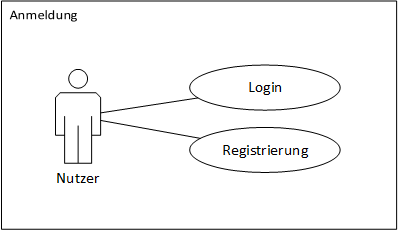
\includegraphics[width=\textwidth]{abb/usecase_login}
\caption{Use Cases der Login Aktivität}
\end{figure}
Während ein Appnutzer ausgeloggt ist, soll ihm keinerlei Funktionalität der App zur Verfügung stehen. Er hat hier also nur die Möglichkeit sich anzumelden oder neu zu registrieren.
\begin {figure}[!hb]\label{fig:usecase_main}
\centering
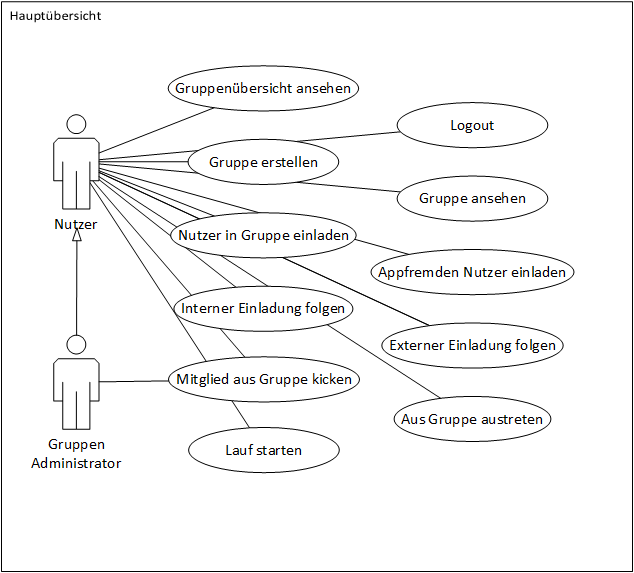
\includegraphics[width=\textwidth]{abb/usecase_main}
\caption{Use Cases der Hauptaktivität}
\end{figure}
Ist der Nutzer eingeloggt und befindet sich nicht in einem Lauf, stehen ihm verschiedene Aktionen zur Verfügung. Er kann hierbei Gruppen verwalten, seine aktuellen Platzierungen ansehen und Läufe starten. Während des Laufens ist diese Funktionalität nicht von Bedeutung, da sich Nutzer hier auf den Sport und sich selbst konzentrieren müssen.
\begin {figure}[!hb]\label{fig:usecase_run}
\centering
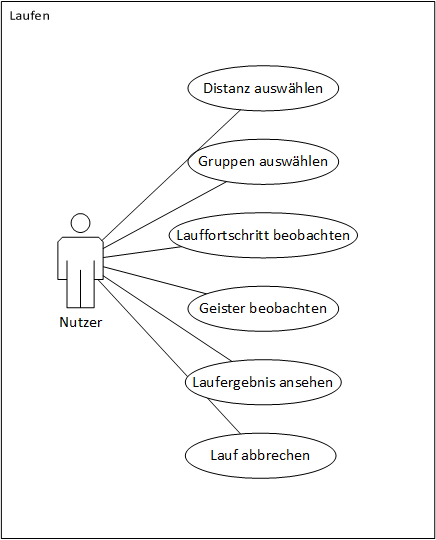
\includegraphics[width=\textwidth]{abb/usecase_run}
\caption{Use Cases der Laufaktivität}
\end{figure}
Soll ein neuer Lauf gestartet werden, muss zunächst die gewünschte Distanz gewählt werden. Danach kann ein Nutzer auswählen, in welchen Gruppen er mit seiner Endzeit antreten möchte und welche Geister angezeigt werden sollen. Die Auswahl einer Gruppe ist hierbei nicht unbedingt notwendig, man kann auch ohne Geister Läufe 
aufzeichnen.
\subsubsection{Beschreibung}
\begin{tabular}{|p{0.2\textwidth}|p{0.8\textwidth}|}
\hline
\textbf{Use Case} & \textbf{Login}  \\ \hline
Aktoren &  Ein Nutzer \\ \hline
Ziel &  Der Nutzer will Zugriff auf die App und seine Daten bekommen \\ \hline
Bedingungen &  Der Nutzer besitzt ein Konto \\ \hline
Beschreibung &  Der Nutzer gibt Name und Passwort an und klickt auf einen Login Button. Die Daten werden an den Server übergeben und von diesem überprüft \\ \hline
Erfolg & Der Server gibt ein Authentifizierungstoken zurück, dass von der App für spätere Netzwerkanfragen gespeichert wird. Die App wechselt zur Hauptansicht  \\ \hline
Misserfolg & Die App zeigt eine Fehlermeldung, die dem Nutzer hilft, sich bei einem erneuten Versuch erfolgreich anzumelden \\ \hline
\hline \end{tabular}
\begin{tabular}{|p{0.2\textwidth}|p{0.8\textwidth}|}
\hline
\textbf{Use Case} & \textbf{Registrierung} \\ \hline
Aktoren &  Ein Nutzer \\  \hline
Ziel &  Der Nutzer will ein neues Konto anlegen, um Zugriff auf die App zu bekommen \\ \hline
Bedingungen &  Keine \\ \hline
Beschreibung &  Der Nutzer gibt seinen gewünschten Nutzernamen, Email und Passwort an und klickt auf einen. Die Daten werden an den Server übergeben und von diesem überprüft und gespeichert \\ \hline
Erfolg & Ein neues Nutzerkonto wird erstellt. Der Nutzer wird eingeloggt und hat Zugriff auf alle Funktionen der App \\ \hline
Misserfolg & Die App zeigt eine Fehlermeldung, die dem Nutzer hilft, sich bei einem erneuten Versuch erfolgreich zu registrieren \\ \hline
\hline \end{tabular}
\begin{tabular}{|p{0.2\textwidth}|p{0.8\textwidth}|}
\hline
\textbf{Use Case} & \textbf{Gruppenübersicht ansehen} \\ \hline
Aktoren &  Ein Nutzer \\ \hline
Ziel &  Der Nutzer will einen Überblick über alle Gruppen bekommen, in denen er sich befindet. \\ \hline
Bedingungen &  Der Nutzer ist angemeldet und befindet sich in der Hauptaktivität\\ \hline
Beschreibung &  Es wird eine Liste aller Gruppen des Nutzers angezeigt. Zusätzlich gibt es Menüpunkte für das Anlegen neuer Gruppen und dem Folgen interner Einladungen \\ \hline
Erfolg & Die Gruppenübersicht wird angezeigt \\ \hline
Misserfolg & Der Nutzer wird abgemeldet, falls eine Authentifizierung nicht möglich ist \\ \hline
\hline \end{tabular}
\begin{tabular}{|p{0.2\textwidth}|p{0.8\textwidth}|}
\hline
\textbf{Use Case} & \textbf{Logout} \\ \hline
Aktoren &  Ein Nutzer \\ \hline
Ziel &  Der Nutzer möchte sich abmelden \\ \hline
Bedingungen &  Der Nutzer ist angemeldet und befindet sich in der Hauptaktivität \\ \hline
Beschreibung & Der Nutzer betätigt den Logout Menüpunkt. Sein Authentifizierungstoken wird genau wie seine Nutzerdaten vom Android Gerät entfernt. Der Anmeldebildschirm wird angezeigt \\ \hline
Erfolg & Der Nutzer hat keinen Zugriff mehr auf die Funktionen der App\\ \hline
Misserfolg & Keiner \\ \hline
\hline \end{tabular}
\begin{tabular}{|p{0.2\textwidth}|p{0.8\textwidth}|}
\hline
\textbf{Use Case} & \textbf{Gruppe erstellen} \\ \hline
Aktoren &  Ein Nutzer \\ \hline
Ziel &  Eine neue Gruppe soll auf dem Server erstellt werden. Der Nutzer soll sich darin befinden \\ \hline
Bedingungen &  Der Nutzer ist angemeldet und befindet sich in der Hauptaktivität. \\ \hline
Beschreibung &  Der Nutzer gibt Gruppenname und die regelmäßig zu laufende Distanz an \\ \hline
Erfolg & Die Gruppe wird erstellt und dem Nutzer angezeigt \\ \hline
Misserfolg & Der Nutzer wird abgemeldet, falls eine Authentifizierung nicht möglich ist \\ \hline
\hline \end{tabular}
\begin{tabular}{|p{0.2\textwidth}|p{0.8\textwidth}|}
\hline
\textbf{Use Case} & \textbf{Gruppe ansehen} \\ \hline
Aktoren &  Ein Nutzer \\ \hline
Ziel &  Der Nutzer möchte die Gruppenmitglieder und ihre Platzierungen ansehen oder die Gruppe verwalten \\ \hline
Bedingungen &  Der Nutzer ist angemeldet und befindet sich in der Hauptaktivität. Er ist Mitglied einer Gruppe \\ \hline
Beschreibung & Die Mitglieder der Gruppe werden in aktueller Reihenfolge angezeigt. Es gibt die Möglichkeit, die Gruppe zu verwalten. Der nächste Stichtag für die Laufauswertung wird angezeigt \\ \hline
Erfolg & Die Gruppenansicht wird angezeigt \\ \hline
Misserfolg & Der Nutzer wird abgemeldet, falls eine Authentifizierung nicht möglich ist \\ \hline
\hline \end{tabular}
\begin{tabular}{|p{0.2\textwidth}|p{0.8\textwidth}|}
\hline
\textbf{Use Case} & \textbf{Nutzer in Gruppe einladen} \\ \hline
Aktoren &  Ein Nutzer \\ \hline
Ziel &  Der Nutzer möchte ein neues Gruppenmitglied einladen \\ \hline
Bedingungen &  Der Nutzer ist angemeldet und befindet sich in der Hauptaktivität. Er ist Mitglied einer Gruppe \\ \hline
Beschreibung & Der Nutzer gibt den gewünschten Nutzernamen in eine Suchmaske ein. Ergebnisse werden ihm angezeigt. Der Nutzer wählt ein Ergebnis aus, woraufhin in der Datenbank eine neue Einladung erstellt wird, die bein Eingeladenen angezeigt wird \\ \hline
Erfolg & Die Einladung wird erstellt und dem Eingeladenen angezeigt \\ \hline
Misserfolg & Kann der gesuchte Name nicht gefunden werden, wird dem Nutzer dies angezeigt. Der Nutzer wird abgemeldet, falls eine Authentifizierung nicht möglich ist \\ \hline
\hline \end{tabular}
\begin{tabular}{|p{0.2\textwidth}|p{0.8\textwidth}|}
\hline
\textbf{Use Case} & \textbf{Appfremden Nutzer einladen} \\ \hline
Aktoren &  Ein Nutzer \\ \hline
Ziel &  Der Nutzer möchte ein neues Gruppenmitglied einladen, dessen Nutzernamen er nicht kennt, oder der die App nicht installiert hat \\ \hline
Bedingungen &  Der Nutzer ist angemeldet und befindet sich in der Hauptaktivität. Er ist Mitglied einer Gruppe \\ \hline
Beschreibung & Der Nutzer betätigt die Teilen Funktion der App. Der Server erstellt eine PIN, die der Gruppe zugeordnet ist. Die PIN kann zusammen mit der Aufforderung, Gh0strunner zu installieren, über beliebige andere Apps versendet werden \\ \hline
Erfolg & Eine PIN wird erstellt und dem Eingeladenen gesendet \\ \hline
Misserfolg & Der Nutzer wird abgemeldet,falls eine Authentifizierung nicht möglich ist \\ \hline
\hline \end{tabular}
\begin{tabular}{|p{0.2\textwidth}|p{0.8\textwidth}|}
\hline
\textbf{Use Case} & \textbf{Interner Einladung folgen} \\ \hline
Aktoren &  Ein Nutzer \\ \hline
Ziel &  Der Nutzer möchte Mitglied einer Gruppe werden, in die er eingeladen wurde \\ \hline
Bedingungen &  Der Nutzer ist angemeldet und befindet sich in der Gruppenübersicht. Er wurde von einem anderen Nutzer eingeladen \\ \hline
Beschreibung & In der Gruppenübersicht wird dem Nutzer eine sonst unsichtbare Option angezeigt, einer neuen Gruppe beizutreten. Akzeptiert der Nutzer die Einladung wird er der Gruppe hinzugefügt \\ \hline
Erfolg & Der Nutzer wird Mitglied der Gruppe \\ \hline
Misserfolg & Der Nutzer wird abgemeldet, falls eine Authentifizierung nicht möglich ist. Er ist kein Mitglied der Gruppe \\ \hline
\hline \end{tabular}
\begin{tabular}{|p{0.2\textwidth}|p{0.8\textwidth}|}
\hline
\textbf{Use Case} & \textbf{Externer Einladung folgen} \\ \hline
Aktoren &  Ein Nutzer \\ \hline
Ziel &  Der Nutzer möchte Mitglied einer Gruppe werden, in die er mit einer PIN eingeladen wurde \\ \hline
Bedingungen &  Der Nutzer ist angemeldet und befindet sich in der Hauptaktivität. Er wurde von einem anderen Nutzer eingeladen \\ \hline
Beschreibung & Der Nutzer gibt eine PIN ein. Diese wird vom Server überprüft und der Nutzer wird zur korrespondierenden Gruppe eingeladen \\ \hline
Erfolg & Der Nutzer wird Mitglied der Gruppe \\ \hline
Misserfolg & Ist die PIN abgelaufen oder ungültig, wird dies dem Nutzer angezeigt. Er wird abgemeldet, falls eine Authentifizierung fehlschlägt. \\ \hline
\hline \end{tabular}
\begin{tabular}{|p{0.2\textwidth}|p{0.8\textwidth}|}
\hline
\textbf{Use Case} & \textbf{Aus Gruppe austreten} \\ \hline
Aktoren &  Ein Nutzer \\ \hline
Ziel &  Der Nutzer möchte Mitglied aus einer Gruppe austreten\\ \hline
Bedingungen &  Der Nutzer ist angemeldet und befindet sich in der Gruppenansicht. Er ist Mitglied einer Gruppe \\ \hline
Beschreibung & Der Nutzer betätigt einen Button. Er wird daraufhin aus der Gruppe entfernt \\ \hline
Erfolg & Der Nutzer ist kein Mitglied der Gruppe mehr \\ \hline
Misserfolg & Der Nutzer wird abgemeldet, falls eine Authentifizierung fehlschlägt. \\ \hline
\hline \end{tabular}
\begin{tabular}{|p{0.2\textwidth}|p{0.8\textwidth}|}
\hline
\textbf{Use Case} & \textbf{Mitglied aus Gruppe Kicken} \\ \hline
Aktoren &  Ein Gruppenadministrator \\ \hline
Ziel &  Der Nutzer möchte Mitglied ein Mitglied aus einer Gruppe entfernen \\ \hline
Bedingungen &  Der Nutzer ist angemeldet und befindet sich in der Gruppenansicht. Er ist Administrator der Gruppe \\ \hline
Beschreibung & Der Nutzer betätigt einen Button. Das zu entfernende Mitglied wird daraufhin aus der Gruppe gelöscht \\ \hline
Erfolg & Das Mitglied ist kein Mitglied der Gruppe mehr \\ \hline
Misserfolg & Das Mitglied wird nicht gelöscht, falls der Nutzer kein Gruppenadministrator ist. Der Nutzer wird abgemeldet, falls eine Authentifizierung fehlschlägt. \\ \hline
\hline \end{tabular}
\begin{tabular}{|p{0.2\textwidth}|p{0.8\textwidth}|}
\hline
\textbf{Use Case} & \textbf{Lauf starten} \\ \hline
Aktoren &  Ein Nutzer \\ \hline
Ziel &  Der Nutzer will einen neuen Lauf starten \\ \hline
Bedingungen &  Der Nutzer ist angemeldet und befindet sich in der Hauptaktivität. Der Lokalisierungsdienst ist aktiviert \\ \hline
Beschreibung &  Es wird eine Auswahl aller möglichen Distanzen und zugehörigen Gruppen angezeigt\\ \hline
Erfolg & Der Dialog zum Starten eines Laufs wird angezeigt \\ \hline
Misserfolg & Der Nutzer wird aufgefordert, den Lokalisierungsdienst zu starten \\ \hline
\hline \end{tabular}
\begin{tabular}{|p{0.2\textwidth}|p{0.8\textwidth}|}
\hline
\textbf{Use Case} & \textbf{Distanz wählen} \\ \hline
Aktoren &  Ein Nutzer \\ \hline
Ziel &  Der Nutzer möchte einen Lauf starten. Dazu muss er als erstes eine Distanz auswählen \\ \hline
Bedingungen &  Der Nutzer ist angemeldet und hat den Menüpunkt Laufen gewählt \\ \hline
Beschreibung & Der Nutzer wählt die gewünschte Distanz aus einem Menü aus. Alle Gruppen der entsprechenden Distanz, in der er sich befindet werden vom Server abgefragt und dem Nutzer angezeigt \\ \hline
Erfolg & Der Nutzer kann Gruppen auswählen und den Lauf starten\\ \hline
Misserfolg & Der Nutzer wird abgemeldet, falls eine Authentifizierung fehlschlägt \\ \hline
\hline \end{tabular}
\begin{tabular}{|p{0.2\textwidth}|p{0.8\textwidth}|}
\hline
\textbf{Use Case} & \textbf{Gruppen auswählen} \\ \hline
Aktoren &  Ein Nutzer \\ \hline
Ziel &  Der Nutzer möchte einen Lauf starten. Nachdem er eine Distanz festgelegt hat muss er alle Gruppen auswählen, in denen er antreten möchte und deren Geister er während des Laufs sehen möchte \\ \hline
Bedingungen &  Der Nutzer ist angemeldet und hat bereits eine Distanz zum Laufen gewählt \\ \hline
Beschreibung & Der Nutzer wählt alle Gruppen aus, in denen er antreten möchte. Beim Start des Laufes werden dann die entsprechenden Geister geladen. Die gewählten Gruppen werden auf dem Gerät gespeichert, um ihnen den Lauf später zuzuordnen \\ \hline
Erfolg & Die Aufzeichnung des Laufs wird gestartet und die gewählten Laufdaten der Geister heruntergeladen \\ \hline
Misserfolg & Der Nutzer wird abgemeldet, falls eine Authentifizierung fehlschlägt \\ \hline
\hline \end{tabular}
\begin{tabular}{|p{0.2\textwidth}|p{0.8\textwidth}|}
\hline
\textbf{Use Case} & \textbf{Lauffortschritt beobachten} \\ \hline
Aktoren &  Ein Nutzer \\ \hline
Ziel &  Der Nutzer läuft, und wird über die vergangene Zeit und zu laufende Strecke informiert \\ \hline
Bedingungen &  Der Nutzer ist angemeldet und hat einen Lauf gestartet \\ \hline
Beschreibung & Die Daten des Laufes werden auf dem Bildschirm ausgegeben und regelmäßig aktualisiert \\ \hline
Erfolg & Die Daten werden angezeigt \\ \hline
Misserfolg & Keiner \\ \hline
\hline \end{tabular}
\begin{tabular}{|p{0.2\textwidth}|p{0.8\textwidth}|}
\hline
\textbf{Use Case} & \textbf{Geister beobachten} \\ \hline
Aktoren &  Ein Nutzer \\ \hline
Ziel &  Der Nutzer läuft, und wird über den Fortschritt der Geister und seine aktuelle Position informiert werden \\ \hline
Bedingungen &  Der Nutzer ist angemeldet und hat einen Lauf mit Geistern gestartet \\ \hline
Beschreibung & Die Daten der Geister und die Nutzerposition werden auf dem Bildschirm ausgegeben und regelmäßig aktualisiert \\ \hline
Erfolg & Die Daten werden angezeigt \\ \hline
Misserfolg & Keiner \\ \hline
\hline \end{tabular}
\begin{tabular}{|p{0.2\textwidth}|p{0.8\textwidth}|}
\hline
\textbf{Use Case} & \textbf{Geister beobachten} \\ \hline
Aktoren &  Ein Nutzer \\ \hline
Ziel &  Der Nutzer ist im Ziel angelangt, und möchte über seine Laufstatistiken informiert werden. Der Lauf soll auf dem Server gespeichert werden \\ \hline
Bedingungen &  Der Nutzer ist angemeldet und hat einen Lauf beendet \\ \hline
Beschreibung & Zielzeit, Strecke und Position des Nutzers werden angezeigt. Der Lauf wird den vorher gewählten Gruppen zugeordnet und hochgeladen. Der Nutzer hat die Möglichkeit, ins Hauptmenü zurückzukehren \\ \hline
Erfolg & Die Daten werden angezeigt \\ \hline
Misserfolg & Keiner \\ \hline
\hline \end{tabular}
\begin{tabular}{|p{0.2\textwidth}|p{0.8\textwidth}|}
\hline
\textbf{Use Case} & \textbf{Geister beobachten} \\ \hline
Aktoren &  Ein Nutzer \\ \hline
Ziel &  Der Nutzer ist im Ziel angelangt, und möchte über seine Laufstatistiken informiert werden \\ \hline
Bedingungen &  Der Nutzer ist angemeldet und hat einen Lauf beendet \\ \hline
Beschreibung & Zielzeit, Strecke und Position des Nutzers werden angezeigt. Er hat die Möglichkeit, ins Hauptmenü zurückzukehren \\ \hline
Erfolg & Die Daten werden angezeigt \\ \hline
Misserfolg & Der Nutzer wird abgemeldet, falls eine Authentifizierung fehlschlägt. \\ \hline
\hline \end{tabular}
\begin{tabular}{|p{0.2\textwidth}|p{0.8\textwidth}|}
\hline
\textbf{Use Case} & \textbf{Lauf abbrechen} \\ \hline
Aktoren &  Ein Nutzer \\ \hline
Ziel &  Der Nutzer möchte den aktuellen Lauf abbrechen \\ \hline
Bedingungen & Der Nutzer ist angemeldet und hat einen Lauf gestartet \\ \hline
Beschreibung & Die Aufzeichnung des Laufs wird auf Knopfdruck abgebrochen, der Nutzer kehrt zum Hauptmenü zurück \\ \hline
Erfolg & Der Nutzer landet im Hauptmenü, der Lauf wird verworfen \\ \hline
Misserfolg & Keiner \\ \hline
\hline \end{tabular}
\begin{tabular}{|p{0.2\textwidth}|p{0.8\textwidth}|}
\hline
\textbf{Use Case} & \textbf{Lauf exportieren} \\ \hline
Aktoren &  Ein Nutzer \\ \hline
Ziel &  Der Nutzer möchte auf seine vergangenen Läufe zugreifen können \\ \hline
Bedingungen & Der Nutzer ist angemeldet und ist bereits gelaufen \\ \hline
Beschreibung & Während des Laufs wird die gelaufene Strecke in einer GPX Datei auf dem Gerät gespeichert. Der Nutzer kann später darauf zugreifen \\ \hline
Erfolg & Eine GPX Datei mit den Daten des Laufs wird erstellt \\ \hline
Misserfolg & Keiner \\ \hline
\hline \end{tabular}
\subsection{Komponenten der Webservers}
Der Webserver dient zur Bereitstellung verschiedener Informationen für die App anhand einer REST-Schnitstelle. 

Im folgenden geht dieses Dokument auf die unterschiedlichen Komponenten des Webservers ein.
\subsubsection{REST API}
\paragraph{Sicherheit}
Um den Zugriff auf die eigenen Daten einzuschränken ist eine Nutzerauthentifizierung nötig. Aufgrund der Zustandslosigkeit, die eine REST-API mit sich bringt, ist die Authentifizierung innerhalb einer Sitzung ausgeschlossen. Nach Definition muss jede Nachricht genügend Informationen enthalten damit der Server die Anfrage verstehen kann, welche durch sitzungsspezifische Informationen stattdessen serverseitig gespeichert werden müssten.

Eine gute Alternative ist hier die Authentifizierung anhand eines Tokens, für die wir uns entschieden haben. Der Client sendet hierbei eine Anfrage an die Authentifierungs-URL an den Server in der Nutzername und Passwort enthalten sind. Sind diese korrekt erhält er ein Token, welches er von da an mit jeder Anfrage an den Server mitschickt.

Dem Token ist eine Lebenszeit zugeordnert. Ist diese überschritten und versucht sich der Nutzer mit dem Token anzumelden erhalt er den HTTP Status ``Unauthorized'' mit Statuscode 401. Dann muss sich erneut authentifiziert werden um ein aktuelles Token zu erhalten.

Für den Rahmen des Projekts haben wir uns auf eine Lebenszeit von drei Tagen festgelegt. Je geringer die Lebenszeit, desto mehr erneute Authentifizierungen durch den Nutzer müssen durchgeführt werden. Das sorgt zwar für höheren Datenverkehr, verkürzt jedoch auch die Zeit, die sich Unbefugte Zugriff verschaffen können, falls sie das Token abgreifen konnten. 
\paragraph{Validierung}
Nutzeranfragen müssen validiert werden um deren Korrektheit zu gewährleisten.

So sind Beschränkungen notwendig, z.B. bei der Passwort- oder Nutzernamenlänge. Auch werden u.A. E-Mail-Adressen validiert, um sie auf die korrekte Form zu prüfen.

Schlägt die Prüfung fehl gibt der Server die Nachricht ``Bad Request'' mit Statuscode 400 zurück, zusammen mit einer aussagekräftigen Nachricht. Das ermöglicht der App diese den Nutzern weiterzugeben um die Korrektur der Eingaben zu vereinfachen.

Die Validierung erfolgt mit dem Java Bean Validation Framework. Dieses ermöglicht annotationsbasierte Validierung von Anfragen.
\subsubsection{Datenspeicherung}
Die lokale Speicherung von Daten auf dem Server ist aus unterschiedlichen Gründen notwendig.

Für eine Authentifizierung ist das persistente Sichern von Nutzerinformationen auf dem Backend-Server nötig. Die sozialen Funktionen erfordern außerdem das zentralisierte Speichern der Läufe, Gruppen und Einladungen.

Um eine organisierte Struktur mit klar definierten Relationen und einen einfach späteren Zugriff zu ermöglichen haben wir uns für die Datenbank MariaDB entschieden, einer performanten quelloffenen SQL-Datenbank.
\paragraph{Bereitstellung der SRTM-Rohdaten}
Um dem Android-Smartphone positionsbezogene Höhendaten bereitzustellen befindet sich ein große Menge an verpackten Höhendaten auf dem Server.

Für jedes Quadrat aus einem Höhen- und einem Breitengrad (welches Informationen enthält) befindet sich auf dem Server eine Zip-komprimierte Datei. Damit entsteht letztendlich eine Dateizahl von 17.387.

Um eine derart große Menge struktur zu bewältigen sind die Dateien in einer Ordnerstruktur der Form <Breitengrad>/<Höhengrad>.zip angelegt.
\paragraph{Externe Einladungen}
Um einer Gruppe neue Nutzer hinzuzufügen benötigt man das Einverständnis des Eingeladenen.

In internen Einladungen, also bei der Einladung von Nutzern der Gh0strunner-App sind diese einfach umsetzbar. Mit einer Gruppen-ID und der ID des Einladenden und des Eingeladenen sind die Einladungen einfach zuzuordnen und der Eingeladene bekommt alle Einladungen innerhalb der App präsentiert.

Da jedoch nicht jeder bereits die App auf dem Smartphone installiert hat ist das Verschicken von Einladungen an Nichtnutzer ein geeigneter Weg um neue Nutzer für die App zu begeistern.

Um externe Nutzer einzuladen ist es jedoch nicht möglich die ID des Eingeladenen zu vergeben, da dieser in der Gh0strunner-Datenbank nicht vorhanden ist.

Stattdessen ist es möglich eine Nachricht mit einer PIN über beliebige andere Apps zu teilen. Diese ist eindeutig einer Einladung zugeordnet. Wird diese in der App eingegeben tritt der Nutzer automatisch der Gruppe bei.
\subsection{Komponenten der Android App}
Die folgenden Abschnitte befasst sich mit der Analyse der Komponenten der Ghostrunner App. Notwendig sind für die Aufzeichnung des Laufes beispielsweise eine Möglichkeit der Positions- und Höhenbestimmung. Es muss außerdem eine Möglichkeit der Authentifizierung und Kommunikation mit dem Webserver geben. Die Android Plattform wird auf mögliche Lösungen untersucht, welche hier beschrieben werden.
\subsubsection{Kommunikation mit dem Webserver}
Für die Kommunikation mit dem Webserver muss eine Internetverbindung zur Verfügung stehen. Diese ist bei allen Geräten, auf denen unsere App laufen soll Standard. Programmatisch wird also nur ein HTTP-Client benötigt, der von der Android-Plattform bereitgestellt wird. Er ermöglicht, dass  HTTP-Anfragen wie GET und POST gestellt werden und Informationen in HTTP-Header und Body übergeben werden können. Beim Warten auf Antworten vom Webserver kommt es automatisch zu nicht vorhersehbaren Verzögerungen. Android erlaubt es aus diesem Grund nicht, diese Netzwerkanfragen im Main Thread der App zu starten, weil sonst während der Wartezeiten die komplette Benutzeroberfläche einfriert. Bei den Standard HTTP-Clients von Android kann die Netzwerkanfrage durch die Benutzung der Klasse AsyncTask in einen separaten Thread ausgelagert werden. \footnote{Connecting to a Network, vgl.~\cite{androidnetwork}}

Vereinfacht werden kann dieser Schritt durch die Benutzung des Android Asynchronous HTTP Client. Die quelloffene Bibliothek bietet einfache funktionen für die HTTP-Anfragen GET, POST, PUT und DELETE, die für die Kommunikation mit RESTful-APIs notwendig sind und empfängt Antworten vom Server automatisch asynchron, wodurch der UI-Thread nicht blockiert wird. \footnote{Android Asynchronous Http Client, vgl.~\cite{loopj}}
\subsubsection{Anmeldung und Authentifizierung}
Ein weiterer wichtiger Aspekt ist die Authentifizierung beim Webserver. Nach einer Anmeldung mit Nutzername und Passwort wird vom Server ein Sicherheitstoken erstellt, das bis zu seinem ebenfalls vom Server definierten Ablaufdatum von Client benutzt werden kann, um sich zu authentifizieren.

Es macht Sinn, diese Authentifizierung an einer einzelnen, dafür dedizierten Stelle im Client zu behandeln. Eine zentrale Speicherung von Anmeldedaten und Sicherheitstoken stellt sicher, dass eine Authentifizierung beim Webserver für alle App-Komponenten möglich ist.

Sobald ein Token abgelaufen ist, ist mit ihm keine weitere Authentifizierung möglich, was durch den HTTP-Statuscode 401 vom Server kommuniziert wird. In diesem Fall muss der die Authentifizierungsstelle der Android App durch erneutes senden der Anmeldedaten einen neuen Token anfordern, woraufhin die ursprüngliche Anfrage wiederholt werden kann.

Bei einem Logout müssen sowohl das aktuelle Authentifizierungstoken, als auch die gespeicherten Nutzerdaten gelöscht werden. Eine Authentifizierung beim Server ist dann erst nach erneuter Anmeldung wieder möglich.
\subsubsection{Positionsbestimmung}
Für eine genaue Laufanalyse muss zu jedem Zeitpunkt die Position des Läufers bekannt sein, denn daraus lassen sich Geschwindigkeit und gelaufene Strecke berechnen. Die Positionsbestimmung erfolgt über das eingebaute GPS-Modul des Smartphones, dessen Genauigkeit in Städten durch WLAN-basierte Ortung und GSM-Ortung durch das Mobilfunknetz verbessert werden kann. Die Module zur Ortung können über das Package android.location der Android API angesprochen werden. Eine Positionsbestimmung ist also mit Boardmitteln eines Android Smartphones ohne Umwege möglich. Eine neuere und verbesserte Möglichkeit bietet die Google Location Services API. Sie ist Teil der Google Play Services, also auf allen Android Geräten verfügbar, die diesen und andere Google Dienste installiert haben, was einem Großteil der Geräte entspricht. Die verschiedenen Ortungsmöglichkeiten werden hier optimiert und zusammengeführt. Programmierer können auf einfache Weise Positionsupdates anfordern und diese über verschiedene Parameter bezüglich Genauigkeit, Updatehäufigkeit und Akkuverbrauch seinen Bedürfnissen anpassen. \footnote{Location Strategies, vgl.~\cite{androidlocation}}
\subsubsection{Höhenbestimmung}
Zusätzlich zu Positions- und Zeitmessung wird für unsere Anwendung noch eine weitere Variable - die Steigung - benötigt. Wenn Läufer verschiedene Strecken laufen, muss diese berücksichtigt werden, um einen fairen Vergleich zu schaffen. Dazu soll später Läufern, die eine größere Steigung überwinden mussten als andere ein Zeitbonus zugesprochen werden.

Für die Bestimmung der Höhe gibt es verschiedene Möglichkeiten, die im Folgenden kurz erläutert werden.
\paragraph{Höhenbestimmung per GPS}
Grundsätzlich ist per GPS eine dreidimensionale Positionsbestimmung möglich, also neben der horizontalen Positionierung auch eine vertikale Höhenmessung. Diese kann jedoch aufgrund der für horizontale Positionsbestimmung optimierten Positionierung der GPS-Satelliten starken Schwankungen unterliegen. Insbesondere in Städten kommt hierzu das Problem der Reflektion des GPS Signals an hohen Gebäuden, durch die die Positionsgenauigkeit weiter beeinträchtigt wird. Die Beeinträchtigung ist horizontal weniger signifikant als vertikal, und wird durch die Nutzung der im vorherigen Abschnitt genannten zusätzlichen Positionierungsmethoden noch weiter optimiert. Vertikal ist eine solche Optimierung nicht möglich. Noch größer ist die Fehlersignifikanz bei dem Versuch, die Höhe über Normalnull zu berechnen, die von dem vom GPS-System genutzten rein mathematischen Ellipsoid WGS-84 abweicht. Durch die Umrechnung vergrößern sich entsprechende Fehler. \footnote{Discussion of vertical GPS Accuracy, vgl.~\cite{gladstone}} Letzteres ist für unsere Arbeit nicht relevant, da wir keine genaue Höhe, sondern nur die relativen Unterschiede für die Steigungsberechnung benötigen. Trotzdem können die möglichen starken Schwankungen der gemessenen Höhe für unsere Anwendung zum Problem werden.
\paragraph{Höhenbestimmung per Web-API}
Für die Höhenbestimmung gibt es die Möglichkeit, verschiedene Web-APIs zu benutzen. Diese geben nach einer HTTP-Anfrage mit übergebenem Längen- und Breitengrad einen Wert für die Höhe an der aktuellen Position zurück. Aufgrund des bereits existierenden HTTP-Klienten wären solche Dienste einfach zu implementieren.

Eine mögliche Variante ist die Google Elevation API. Sie unterliegt allerdings neben einer maximalen Anfragemenge pro Tag der Restriktion, dass sie nur in Verbindung mit einer Darstellung auf Google Maps verwendet werden darf.\footnote{The Google Elevation API, vgl.~\cite{googleelevation}}  Da unsere App ohne Karte funktionieren soll und keinerlei Navigation anbieten, sondern lediglich Läufe aufzeichnen soll, fällt diese Möglichkeit deshalb aus.

Eine Alternative ist die Benutzung der MapQuest Elevation API. Die Benutzung dieses Service ist frei, käme also für unsere Anwendung in Frage. Dennoch kann sich durch die Abhängigkeit von einem fremden Service ein Skalierungsproblem ergeben, wenn sich die Nutzerzahl unserer App vergrößert. \footnote{MapQuest Open Elevation API Web Service, vgl.~\cite{mapquest}}

Eine weitere Möglichkeit wäre, den Webservice mithilfe der im nächsten Abschnitt beschriebenen SRTM-Rohdaten auf unserem Webserver selbst zu implementieren.

Bei Benutzung einer Web-API entsteht für unsere Anwendung generell ein signifikanter Nachteil. Eine Internetverbindung müsste zu jeder Zeit gewährleistet sein, was insbesondere bei Läufen in abgelegenen Gebieten nicht immer der Fall ist. Dieses Problem steht der gewünschten Echtzeit-Aufzeichnung des Laufes im Weg.
\paragraph{Höhenbestimmung per SRTM-Rohdaten}
Auf der NASA Shuttle Radar Topographic Mission (SRTM) wurden Höhendaten vom gesamten Globus gesammelt. Die horizontale Auflösung der Daten beträgt 90 Meter, die vertikale Genauigkeit der Daten mindestens 16 Meter. Die relativen Höhenunterschiede in zusammenhängenden Bereichen sollte aber meist deutlich niedriger sein. Die Daten stehen für die gesamte Erdoberfläche zum Download bereit. Einzelne Kacheln decken dabei 5 Grad Länge x 5 Grad Breite ab, das entspricht in beiden Richtungen ca. 550 Kilometer. Es ergibt sich eine Dateigröße von ca. 200 Megabyte pro Kachel, als Zip gepackt kann diese auf eine Größe von ca. 1 bis 20 Megabyte verkleinert werden. 
\footnote{SRTM 90m Digital Elevation Database v4.1, vgl.~\cite,{srtm}}
Die Daten liegen im Dateiformat Arcascii vor, das ähnlich einer CSV-Datei aufgebaut ist:
 \begin{lstlisting}[frame=htrbl, caption={Beispiel Arcascii Datei}, breaklines=true]
ncols 6000
nrows 6000
xllcorner 10
yllcorner 45
cellsize 0.00083333333333333
NODATA_value -9999
-9999 1 2 3
4 5 6 7
8 9 10 11
12 13 14 15
\end{lstlisting}
Die ersten sechs Zeilen geben Informationen über die Form der Datei an. Ncols und nrows bezeichnen hierbei die Anzahl der Zeilen und spalten der Datei. Bei einer Auflösung von 90 Metern und einer Abdeckung von 550 Kilometern pro Richtung ergibt das jeweils 6000 Zeilen und Spalten, die unter den Headerinformationen beginnen. Xllcorner und yllcorner bezeichnen, auf welcher Koordinate des WGS84 Koordinatensystems sich die untere linke Ecke der Datei befindet. In unserem Beispiel würde diese Koordinate der Höhe 12m entsprechen. Cellsize beschreibt, wie groß die Abstände zwischen den angegeben Punkten sind. 0.00083 Grad entsprechen dabei ca. 90 Metern. 
\footnote{ESRI ASCII Raster format, vgl.~\cite,{esri}}

Um das Höhenprofil für Läufe selbst zu berechnen, muss unsere App die für den Standort des Nutzers relevanten Kacheln herunterladen und die der aktuellen Position entsprechenden Stelle in der Datei finden. Da für einzelne Läufe keine 550x550km abgedeckt werden müssen, sondern ein wesentlich kleinerer Bereich benötigt wird, lässt sich durch eine Aufteilung der Dateien eine für das Mobilfunknetz akzeptable Dateigröße erreichen.

Am Anfang jedes Laufs würden dann alle für die aktuelle Position des Läufers notwendigen Dateien heruntergeladen und auf dem Gerät gespeichert werden. Wenn die Daten auf unserem Webserver bereitliegen, sind wir von keinem externen Service mehr abhängig. Die App kann dann selbstständig für jeden während des Laufs aufgezeichneten Punkt die entsprechende Höhe aus der Datei extrahieren. Die Methode hat den Vorteil, dass nach einem einmaligen Herunterladen der Höhendaten kein weiterer Internetzugriff mehr benötigt wird. Außerdem bleiben die Dateien auf dem Gerät gespeichert, das heißt Läufe in der gleichen Umgebung können ohne einen erneuten Download stattfinden.

Um Steigungsunterschiede auch kleinschrittiger als alle 90 Meter festzustellen, müssen die Höhenwerte interpoliert werden. Es werden dabei die nächsten 4 Punkte mit Höhenwert entsprechend ihrem Abstand zum Nutzer gewichtet, und so eine Mittelwert errechnet. Aus diskreten Werten kann so eine geglättete Kurve errechnet werden.
\paragraph{Kombination verschiedener Methoden}
Insbesondere durch Kombination von GPS und und Nutzung der SRTM Daten sollten sich sehr genaue Ergebnisse erzielen lassen. Die Implementierung des Höhenbestimmungsmoduls sollte also flexibel genug sein, um das zuzulassen. Erreicht wird diese Flexibilität durch die Implementierung eines Interfaces ElevationService, das die Methode getElevation(double latitude, double longitude) besitzt. Durch Nutzung dieses Interfaces können verschiedene Services einfach ausgetauscht oder mit wenig zusätzlichem Programmieraufwand kombiniert werden. Hier muss nur noch ein Algorithmus entwickelt werden, der bestimmt, auf welche Weise verschiedene Höhendaten kombiniert werden. Für die Studienarbeit haben wir uns explizit für die Implementierung der SRTM Methode entschieden, Veränderungen in späteren Versionen sind durch das Interface jederzeit ohne großen Aufwand möglich.
\subsubsection{Aufzeichnen des Laufes}
Für die Aufzeichnung des Laufes sind nun alle wichtigen Voraussetzungen geschaffen. Nach regelmäßigen Positionsupdates werden die zugehörigen Höhendaten abgefragt. Daraufhin kann die zurückgelegte Strecke schrittweise im Vergleich zur seit Laufbeginn vergangenen Zeit berechnet werden. Ist die vorgegebene Laufstrecke erreicht, gilt dieser als beendet.

Zusätzlich zur Berechnung der zurückgelegten Strecke werden die aufgezeichneten Wegpunkte bei jedem Positionsupdate in eine GPX-Datei geschrieben. Jeder Wegpunkt enthält einen Zeitstempel, Längen- und Breitengrad, sowie die aktuelle Höhe.

Eine Variante, um einen Ausgleich zwischen verschieden steilen Strecken zu schaffen ist es, statt der Zielzeit eine unabhängig davon errechneten Punktzahl für den Vergleich der Läufer heranzuziehen. Diese würde in steilen Streckenabschnitten schneller erhöht werden als in flachen.

Um die App für den Benutzer aber möglichst simpel und durchsichtig zu halten, haben wir uns für eine andere Methode entschieden. Hierbei wird für jeden Abschnitt zwischen zwei Positionsupdates ein Multiplikator errechnet. Auf steilen Strecken wird der zurückgelegte Weg mit einer Zahl größer als eins multipliziert, der Läufer kommt also entsprechend früher ins Ziel. Läuft er bergab, erst etwas später. Auf einer Strecke von beispielsweise einem Kilometer mit konstanter Steigung, für die ein Multiplikator von 1,1 errechnet wurde, würde der Nutzer sein Ziel also schon nach 909 Metern erreichen.

Der Vergleich mit anderen Läufern ist in dieser Variante sehr einfach möglich, denn der Abstand zu den Geistern kann zu jedem Zeitpunkt in Metern angegeben werden. Bei einer willkürlich gewählten Punktzahl wäre dieser für den Nutzer schwieriger nachzuvollziehen.

Zunächst ist noch unklar, wie groß der Multiplikator sein muss, um einen fairen Vergleich zu schaffen. Eine genaue Berechnung kann sicher erst nach ausführlichen Tests gefunden werden. Auch dann sind perfekte Multiplikatoren unwahrscheinlich, denn jeder Läufer reagiert unterschiedlich auf verschiedene Steigungen.

Sicher ist, dass auch ein Teil der vergangenen Strecke für die Berechnung herangezogen werden muss, denn eine moderate Steigung über längere Zeit zu überwinden kann schwieriger sein, als über einen sehr kurzen Zeitraum mit extremer Steigung zu laufen.
\subsubsection{Darstellung des Laufes}
Für die Darstellung des Laufes muss ein eigenes UI Element gestaltet werden. Informationen wie der aktuelle Fortschritt in Metern und Prozent, die verbleibende Strecke und die vergangene Zeit seit Beginn des Laufes müssen hier ansprechend und wiedererkennbar dargestellt werden.

Zusätzlich muss eine Vergleich zu vorher gelaufenen Mitstreitern möglich sein, eine grafische Fortschrittsanzeige sollte also den aktuellen Läufer im direkten Vergleich mit möglichen Geistern anzeigen. Eine Positionsanzeige ist hier zusätzlich sinnvoll.
\subsubsection{Frontend der Android App}
Andere Elemente der Benutzeroberfläche sollten sich mit Standard UI Elementen des Android Systems, wie Buttons, Textfeldern und Auswahllisten darstellen lassen. Wichtig ist hier ausßerdem ein globales Hauptmenü, über dass sich in Gruppenansichten wechseln oder Läufe starten lassen.

\section{Design}\label{kapitel5}
\subsection{Datenbank}
\begin{figure}[!h]
\centering
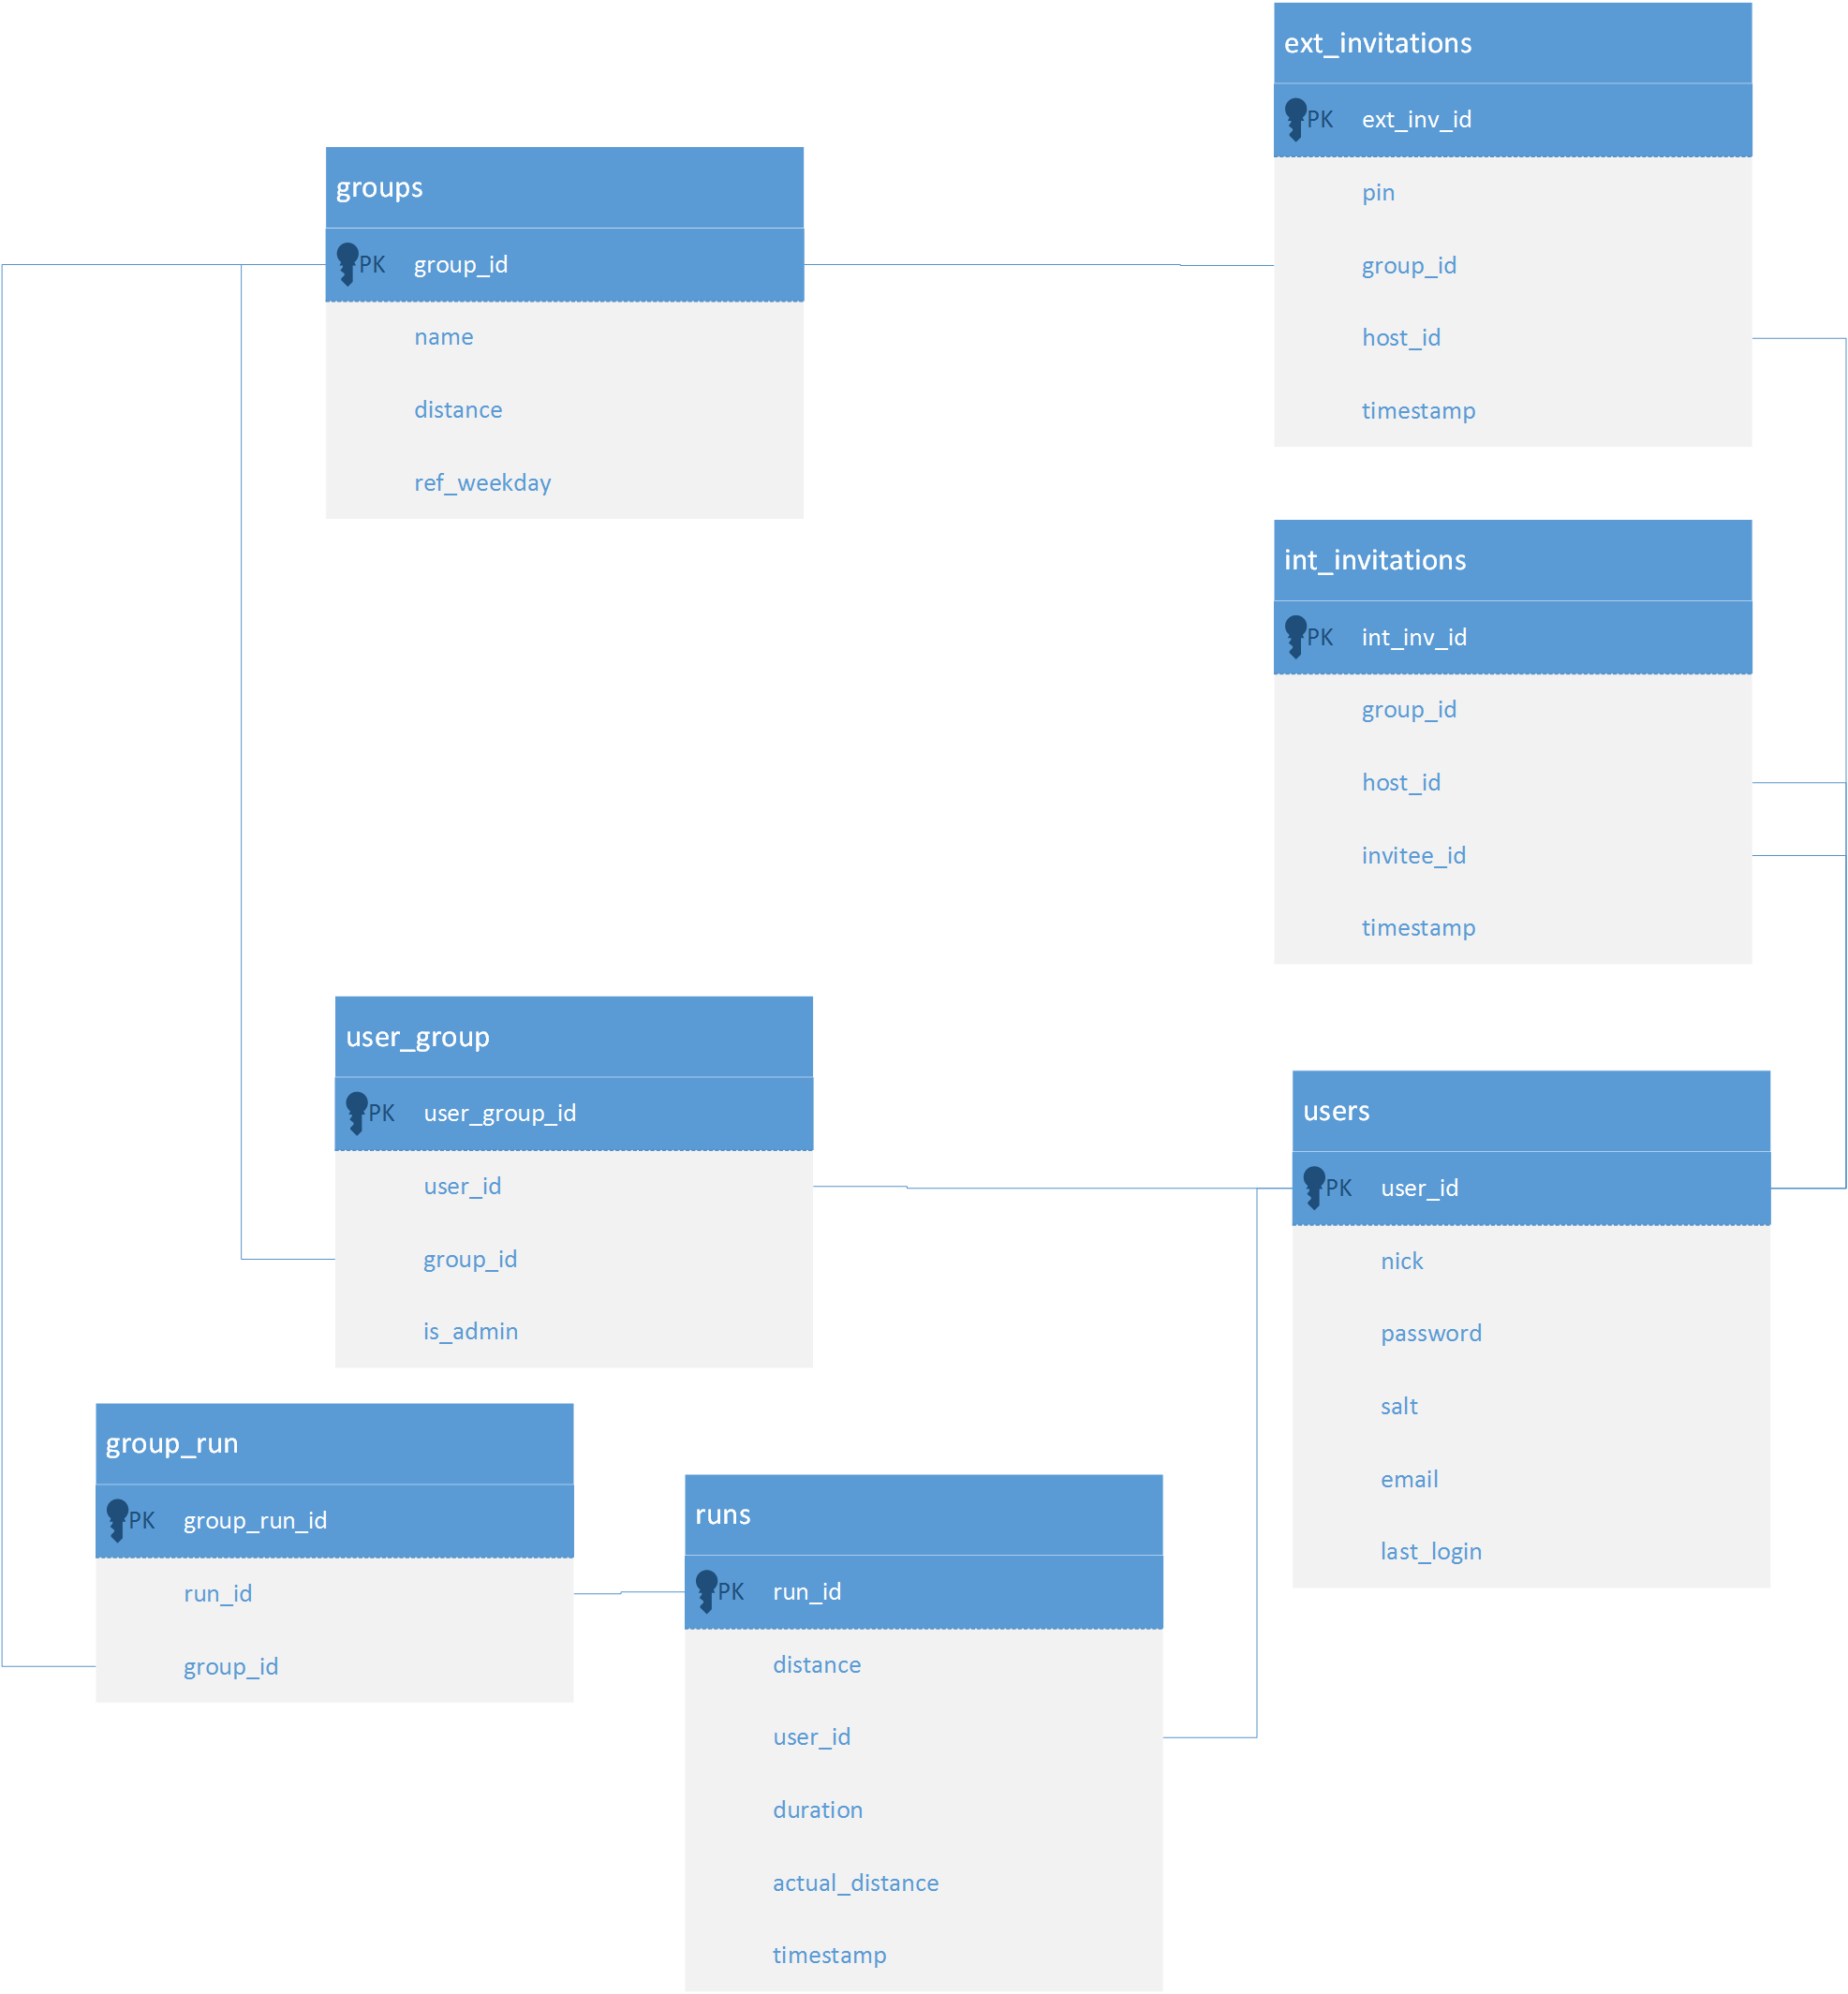
\includegraphics[width=\textwidth]{abb/er_diagram}
\caption{Datenbankschema}
\end{figure}
Die Datenbank besteht aus Tabellen für den Nutzer, die Gruppen, internen als auch externen Einladungen und den Läufen. Zusätzlich bestehen zwei weitere Tabellen für das Abbilden von n:m-Beziehungen.

Jeder Tabelle ist ein Primärschlüssel zuegordnet um eine eindeutige Identifikation jedes Tupels zu ermöglichen.

Jedem Nutzer ist ein einzigartiger Nutzername, ein verschlüsseltes Passwort, ein Salt für die Hashingfunktion, eine E-Mail-Adresse und ein Zeitstempel des letzten Logins zugeordnet.

Eine Gruppe besteht aus dem Namen, der vorgegebenen Laufdistanz und einem wöchtentlichen Stichtag, zu dem die Läufe der davorliegenden Woche ausgewertet werden. Dieser besteht aus einer Ganzkommazahl zwischen null und sechs, welche die Wochentage beginnend mit Sonntag enumeriert.

Es kann eine unbegrenzte Anzahl an Nutzern einer Gruppe beitreten und Nutzer können beliebig vielen Gruppen beitreten. Es handelt sich also um eine n:m-Relation, die anhand der Tabelle user\_group dargestellt ist. Zusätzlich wird in user\_group festgehalten, ob es sich bei dem Nutzer um einen Gruppenadministratoren handelt. Hier steht die ``1'' für ``Admin'' und die ``0'' für ``Nichtadmin''.

Eine weitere n:m-Relation mittels der Tabelle group\_run zwischen Läufen und Gruppen. Dem Lauf sind die Attribute Distanz, Nutzer-ID, Dauer, die wirkliche Distanz und ein Zeitstempel zugeordnet. Die Nutzer-ID stellt eine 1:1-Beziehung auf den Nutzer dar.

Des weiteren wurden die Tabellen ext\_invitations und int\_invitations angelegt.

Externe Einladungen sind Einladungen an Andere außerhalb der App. Es wird eine PIN geteilt, mit dem der Eingeladene später die Einladung annehmen kann. Diese ist eine 10-stellige Ganzkommazahl, Außerdem befinden sich in der Tabelle die Gruppen-ID und die Nutzer-ID, welche jeweils 1:1-Beziehungen markieren sowie ein Zeitstempel.

Interne Einladungen gehen an andere Nutzer der App. Hier sind die Attribute die ID des Einladenden, des Eingeladenen und der Gruppe. Außerdem besteht auch hier ein Zeitstempel.
%TODO Logout-->Login/Register, Kick User ist keine eigene Seite, kick nur wenn admin
\subsection{Navigationsschema}
\begin{figure}[!h]
\centering
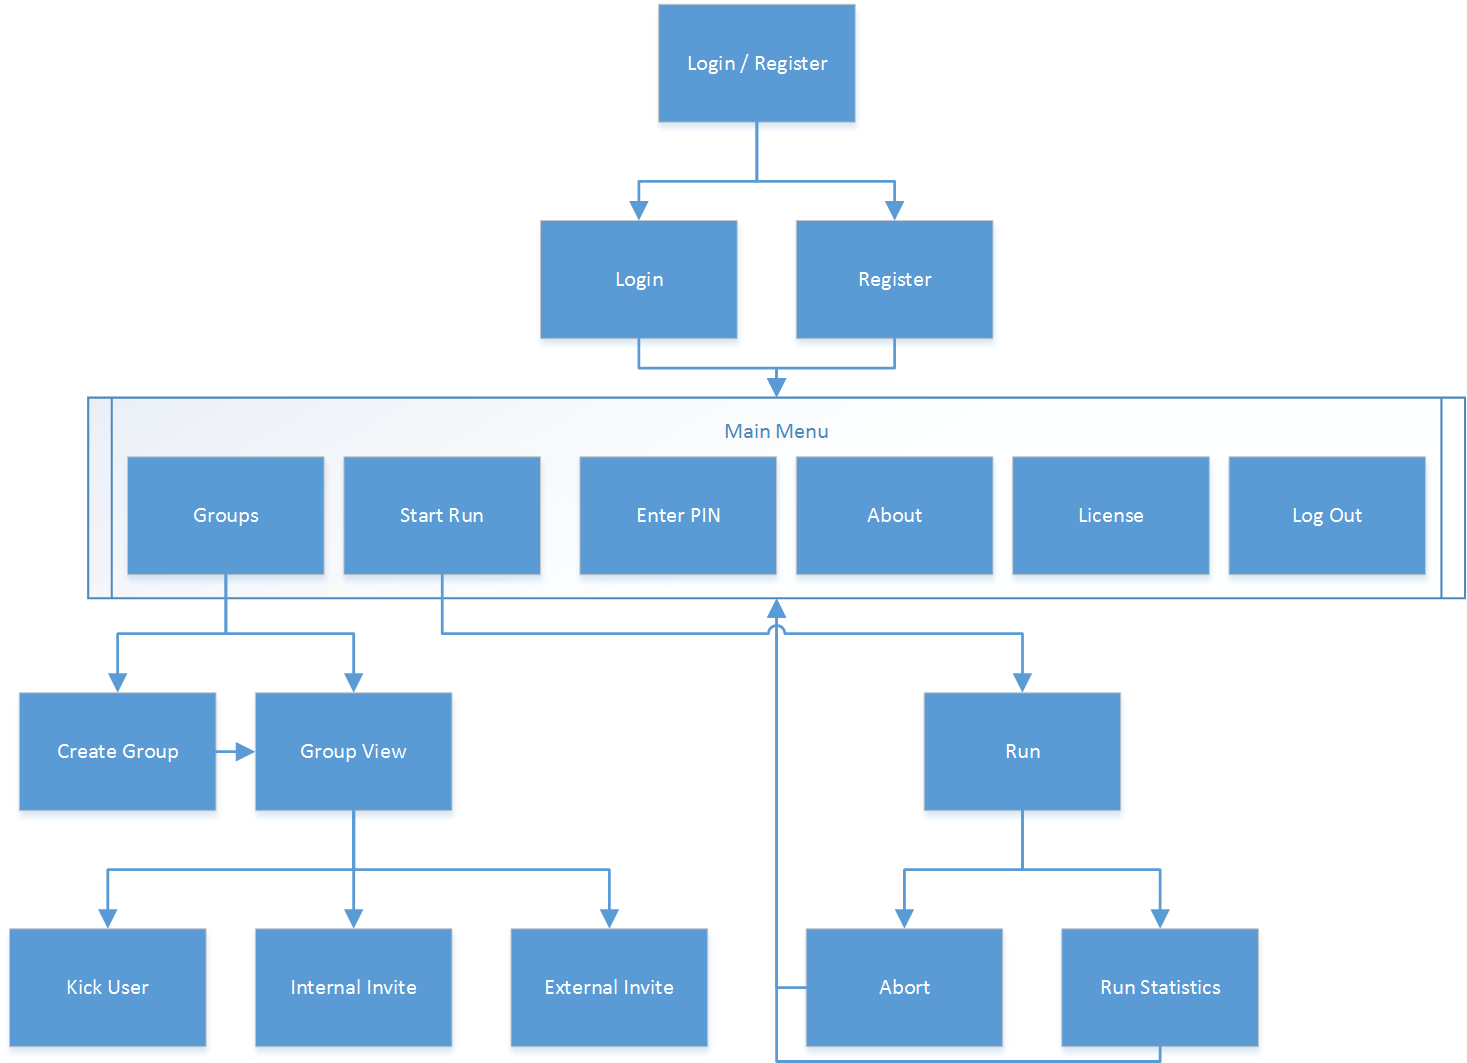
\includegraphics[width=\textwidth]{abb/navigation_diagram}
\caption{Navigationsdiagramm}
\end{figure}

%Warum was wo und wie
Nach dem Anmelden bzw. Registrieren befindet sich der Nutzer in der Gruppenübersicht. Diese ist Teil des Navigationsmenüs. Aus diesem lassen sich alle wichtigen Funktionalitäten erreichen:
\begin{itemize}
\item Gruppenübersicht - Auflistung der eigenen Gruppen und der Einladungen in Gruppen
\item Laufen - Erster Schritt zum Start des Laufs. Es wird dem Nutzer die Wahl gegeben für welche Gruppen er laufen möchte bzw. auf welcher Distanz.
\item PIN-Eingabe - Eingabe der PIN, die der Nutzer bei einer externen Einladung erhält.
\item Über - Hier stehen kurze Informationen über das Team.
\item Lizenz - Hier befindet sich die Lizenz unter der die App steht; die GNU Public License. 
\item Abmelden - Hier kann sich der Nutzer abmelden, um zurück zur Anmeldung / Registrierung zu gelangen.
\end{itemize}

Das Hauptmenü ist ein seitliches Menü, welches durch Drücken des Stapel-Icons in der oberen linken Ecke oder durch Hereinwischen vom linken Bildschirmrand erreichbar ist.
\begin{figure}[!h]
\centering
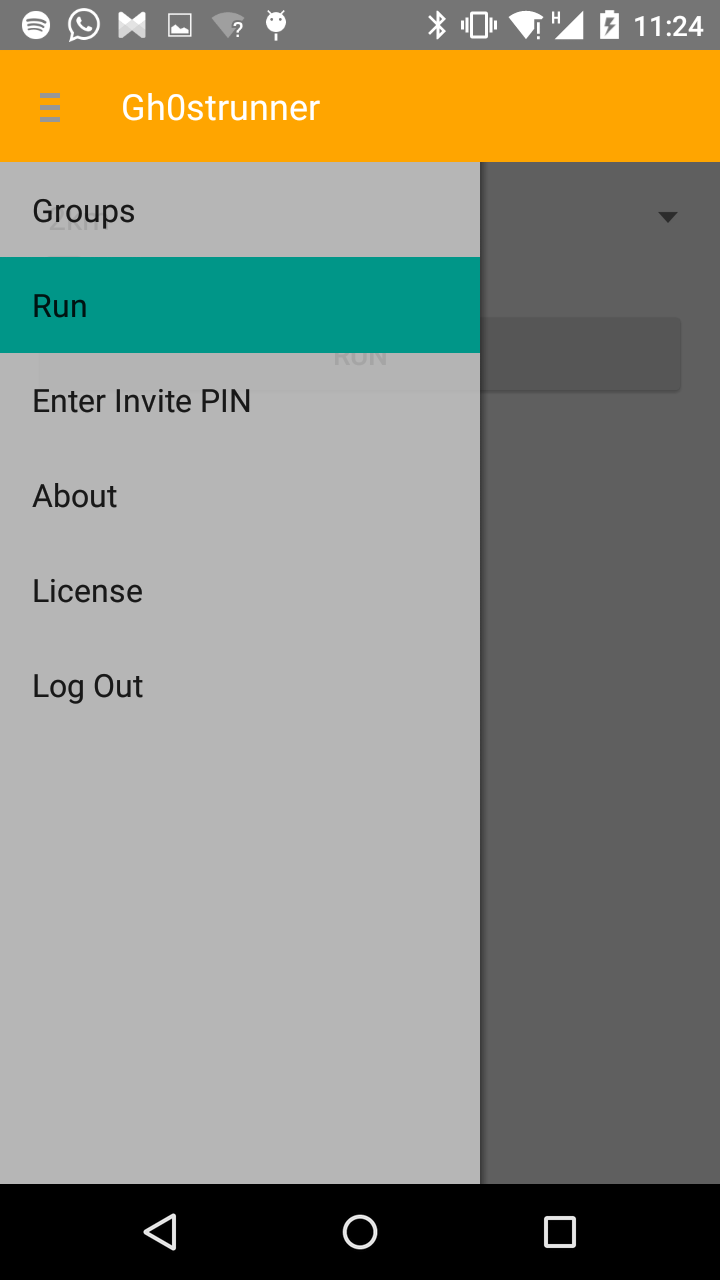
\includegraphics[width=0.3\textwidth]{abb/bsp/bsp7}
\caption{Aufgeklapptes Hautpmenü}
\end{figure}

Wir haben uns für das Menü entschieden um unnötige Komplexität und Tiefe der Navigation zu vermeiden, was sowohl den Aufwand beim Programmieren der App als auch die Benutzung vereinfacht.
\subsection{Motivation}
Für viele Menschen macht Sport keinen Spaß, es ist etwas wozu sie sich zwingen müssen. Aber auch für erfahrene Athleten ist es manchmal schwierig, sich zu motivieren. Genau hier soll unsere App ansetzen, um Nutzern die Chance zu geben, sich wieder auf's Laufen zu freuen, anstatt es als Aufgabe zu sehen. Wir haben einige Punkte gesammelt, die die Motivation, zu Gh0strunner zurückzukehren erhöhen sollen.

Ein Beispiel ist die Darstellung von Geistern. Durch sie soll der läufer angespornt werden, während des Laufs sein Bestes zu geben. Am Ende des Laufs nochmal alles zu geben, um auf dem ersten Platz zu landen oder ihn zu halten, kann eine besser Motivation darstellen, als ein abstraktes "damit es einem danach besser geht".

Die Motivation soll auch zwischen den Läufen anhalten. Dafür kann der Nutzer jederzeit die vergangenen Läufe der Gruppenmitglieder ansehen und wird zusätzlich angetrieben, wenn er sieht, dass sein bester Freund gerade eine bessere Zeit gelaufen ist.

Auch funktionale Aspekte müssen für erfolgreiche Umsetzung unseres Ziels bedacht werden. Durch volle und aktive Gruppen wird der Spaß bei der Benutzung unserer App erhöht. Gruppen sollten außerdem genau einer Lauflänge zugeordnet werden, damit Nutzer stets den Überblick behalten und Gruppen wählen, in denen sie auch aktiv sind. Es macht keinen Sinn, als Anfänger einmal pro woche 20 Kilometer zu laufen. Ein sinnvoller Schritt um Gruppenbildung zu unterstützen ist es deshalb, die Anzahl der unterschiedlichen Lauflängen einzuschränken. Wir haben uns für mögliche Lauflängen von 2km, 5km, 8 km, 10km, 15km und 20km entschieden. Eine kleinschrittigere Aufteilung würde die Appnutzer auf zu viele Gruppen verteilen, wobei sie in jeder einzelnen Gruppe wahrscheinlich weniger aktiv wären.
\subsection{Laufoberfläche}
Um die Wiedererkennbarkeit und Attraktivität einer App zu haben, lohnt es sich unikate Benutzeroberflächenelemente einzusetzen. Die Stelle, an der das für unsere App sinnvoll ist, ist während des Laufens, da alle restlichen Oberflächen hauptsächlich der Verwaltung dienen.

Wir haben uns für eine kreisförmige Darstellung der Strecke entschieden, da so einerseits der Bildschirm von Smartphones am besten ausgenutzt wird, und gleichzeitig die Assoziation zu einer runden Stadionstrecke mit Start- und Zielline geweckt wird.

Ein farbiger Kreis soll dabei den Nutzer darstellen, der sich im Verlauf des Laufes einmal über die dargestellte Strecke bewegt. Geister werden als kleinere Kreise dargestellt, die sich mit der dauerhaft Durchschnittsgeschwindigkeit ihres Laufes bewegen. Die Abweichung der eigentlichen Laufgeschwindigkeit zur Durchschnittsgeschwindigkeit sollte bei korrekter Wahl des Steigungsmultiplikators sowieso relativ gering sein, denn dieser soll optimalerweise die zusätzliche Anstrengung durch die Steigung ausgleichen. So kann bei der Darstellung der Geister einiges an Berechnungen eingespart werden, denn es wird nur die Zielzeit jedes Geistes benötigt.

\begin {figure}[!h]\label{fig:runscreen}
\centering
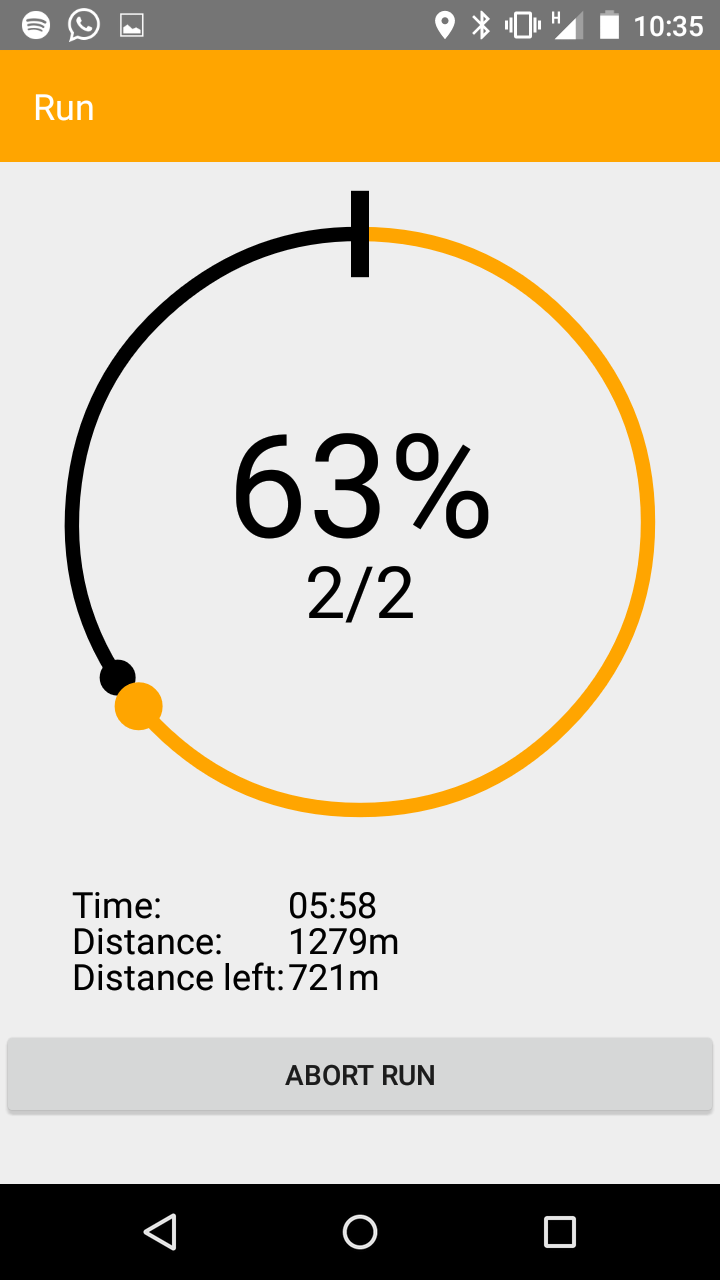
\includegraphics[width=0.4\textwidth]{abb/bsp/bsp19}
\caption{Anzeige des Laufs mit Geist in Gh0strunner}
\end{figure}

Im Kreis kann der Lauffortschritt, und die aktuelle Position des Läufers gegenüber den Geistern angezeigt werden. Unter dem Kreis ist dann noch Platz für zusätzliche Laufstatistiken. 

Eine Kartendarstellung wäre ebenfalls denkbar. Wir haben uns gegen sie entschieden, da sie wo keine vorgegeben Strecke existiert sowieso nur bedingt sinnvoll wäre. Außerdem ergäbe sich durch die fehlende Möglichkeit einer ansprechenden Darstellung der Geister ein optischer Nachteil.
\subsection{Logo}
Um den Wiedererkennungswert der App zu erhöhen wurde ein Logo entworfen, welches den Inhalt wiederspiegeln sollte.

Der erste Entwurf erwies sich nach einer kleinen Umfrage als zu infantil.

\begin{figure}[!h]
\centering

\includegraphics[width=0.3\textwidth]{abb/icon_entwurf1}
\caption{Logo Entwurf 1}
\end{figure}
Der zweite Entwurf war etwas langweilig und zu hoch im Vergleich zu Bildbreite. 

\begin{figure}[!h]
\centering

\includegraphics[width=0.3\textwidth]{abb/icon_entwurf2}
\caption{Logo Entwurf 2}
\end{figure}
Letztendlich haben wir uns für den dritten Entwurf als App-Icon entschieden, da es Zuspruch unter den Befragten gefunden hat. Außerdem enthält es G und R aus \textbf{G}h0st\textbf{r}unner und entspricht den quadratischen Vorgaben.
\begin{figure}[!h]
\centering

\includegraphics[width=0.3\textwidth]{abb/icon_entwurf3}
\caption{Logo Entwurf 3}
\end{figure}

\subsection{Aufbau der REST-API}
\subsubsection{URLs und erlaubte Anfragen}
Die folgende Tabelle dient dem Überblick, welche Ressourcen über die REST-API abfragbar sind und welche HTTP-Operationen auf diesen erlaubt sind.
\begin{center}
\begin{longtable}{| p{4.1cm} | p{2cm} | p{2cm} | p{2cm} | p{2cm} |}
\hline
Relative URL  & GET & POST & PUT & DELETE \\ 
\hline \hline
/user & Auflistung aller Nutzer & Anlegen eines Nutzers &  & \\
\hline
/user/<id> & Abfrage eines Nutzers & & Nutzer wird ersetzt & Löschen eines Nutzers \\
\hline
/user/<id>/run & Auflistung aller Läufe & Anlegen eines Laufs & & \\
\hline
/user/<id>/\-run/<id> & Abfrage eines Laufs & & & Löschen eins Laufs \\
\hline
/user/<id>/group & Abfrage der Gruppen in denen der Nutzer Mitglied ist & & & \\
\hline
/group & Auflistung aller Gruppen & Anlegen einer Gruppe & & \\
\hline
/group/<id> & Abfrage einer Gruppe & & & Löschen einer Gruppe \\
\hline
/group/<id>/user & Auflistung aller Gruppenmitglieder & Zufügen eines Nutzers zur Gruppe & & \\
\hline
/group/<id>/\-user/<id> & Abfrage eines Gruppenmitglieds & & & Austritt des Nutzers aus der Gruppe \\
\hline
/group/<id>/admin & Abfrage des Gruppenadministrators & & & \\
\hline
/group/<id>/\-run/current & Abfrage aller Läufe in der Gruppe nach dem letzten Stichtag & & & \\
\hline
/extinvite & Auflistung aller externen Einladungen & Anlegen einer externen Einladung & & \\
\hline
/extinvite/<id> & Abfrage einer externen Einladung & & & \\
\hline
/user/<id>/\-extinvite/accept/<pin> & & Annehmen der Einladung an den Nutzer & & \\
\hline
/user/<id>/intinvite & Abfrage aller Einladungen an den Nutzer & Anlegen einer Einladung an den Nutzer & & \\
\hline
/user/<id>/\-intinvite/<id> & & & & Löschen bzw. Ablehnen einer internen Einladung \\
\hline
/tile/<breite>/<hoehe> & Download der SRTM-Datei für den Höhen- und Breitengrad & & & \\
\hline
/login & & Anmelden des Nutzers um ein Sicherheitstoken zu erhalten & & \\
\hline
\end{longtable}
\end{center}

\subsubsection{Aufbau der Anfragen}
\paragraph{GET}
Alle GET-Anfragen haben einen leeren Request Body. Alle nötigen Informationen sind in der URL enthalten.

\paragraph{POST}
Die POST-Anfragen werden in Form von JSON übertragen und dienen dazu neue Ressourcen anzulegen. 

Die folgende Tabelle gibt eine Übersicht in welcher Form Anfragen getätigt werden können. ``<>'' ist ein Platzhalter für den jeweiligen Wert.

Die Reihenfolge der JSON-Attribute ist unwichtig.

\begin{center}
\begin{longtable}{| p{4.1cm} | p{5cm} | p{3cm} |}
\hline
URL & Form der Anfrage & zusätzliche Informationen \\
\hline \hline
/user & \{ ``nick'':``<>'', ``password'':``<>'', ``email'':``<>'' \} & \\
\hline
/user/<id>/run & \{ ``distance'':``<>'', ``duration'':``<>'', ``actualDistance'':``<>'', ``groupIDs'':[<>, ...] \} & Eine oder mehrere Gruppen-IDs sind möglich\\
\hline
/group & \{ ``name'':``<>'', ``admin'':``<>'', ``distance'':``<>'' \} & ``admin'' enthält einer Nutzer-ID \\
\hline
/group/<id>/user & \{ ``userID'':``<>'' \} & \\
\hline
/extinvite & \{ ``hostID'':``<>'', ``groupID'':``<>'' \} & \\
\hline
/user/<id>/intinvite & \{ ``hostID'':``<>'', ``groupID'':``<>''] \} & \\
\hline
/login & \{ ``name'':``<>'', ``password'':``<>'' \} & \\
\hline
/user/<id>/extinvite/\-accept/<pin> & & \\
\hline
\end{longtable}
\end{center}
\paragraph{PUT}
Die Methode PUT wurde nur an einer Stelle implementiert. Sie dient dazu einen existierenden Eintrag zu ersetzen.

\begin{center}
\begin{longtable}{| p{4.1cm} | p{5cm} | p{3cm} |}
\hline
URL & Form der Anfrage & zusätzliche Informationen \\
\hline \hline
/user/<id> & \{ ``nick'':``<>'', ``password'':``<>'', ``email'':``<>'' \} & \\
\hline
\end{longtable}
\end{center}

\paragraph{DELETE}
Alle DELETE-Anfragen haben einen leeren Request Body. Die nötigen Informationen wie z.B. IDs befinden sich in der URL.

\subsubsection{Aufbau der Antworten}
Im folgenden befindet sich eine Auflistung der Form der Antworten, die der Server nach Anfragen des Servers zurückschickt.

\paragraph{GET}
\begin{center}
\begin{longtable}{| p{4.1cm} | p{10cm} |}
\hline
URL & Form der Serverantwort \\
\hline \hline
/user & ``[\{``userID'':<>, ``nick'':``<>'', ``email'':``<>''\}, \{..\}, ..] \\
\hline
/user/<id> & \{``userID'':<>, ``nick'':``<>'', ``email'':``<>''\} \\
\hline
/user/<id>/run & [\{"runID":<>,"distance":<>,"duration":<>,\-"actualDistance":<>,"timestamp":<>,"groups":\-[\{"groupID":<>,"name":"<>","distance":<>,\-"refWeekday":<>,"users":null\}]],"user":\-\{"userID":<>,"nick":"<>","email":"<>"\}\}, \{..\}, ..] \\
\hline
/user/<id>/\-run/<id> & \{\{"runID":<>,"distance":<>,"duration":<>,\-"actualDistance":<>,"timestamp":<>,"groups":\-[\{"groupID":<>,"name":"<>","distance":<>,\-"refWeekday":<>,"users":null\}],"user":\-\{"userID":<>,"nick":"<>","email":"<>"\}\} \} \\
\hline
/user/<id>/group & \{[\{"groupID":<>,"name":"<>","distance":<>,\-"refWeekday":<>,"users":null\}] \} \\
\hline
/group & \{[\{"groupID":<>,"name":"<>","distance":<>,\-"refWeekday":<>,"users":[\{"userID":<>,"nick":"<>",\-"email":"<>"\}]\}, \{...\}, ...] \} \\
\hline
/group/<id> & \{\{"groupID":<>,"name":"<>","distance":<>,"\-refWeekday":<>,"users":[\{"userID":<>,"nick":"<>",\-"email":"<>"\}]\}\} \\
\hline
/group/<id>/user &  [\{``userID'':<>, ``nick'':``<>'', ``email'':``<>''\}, \{...\}, ...] \\
\hline
/group/<id>/\-user/<id> &  \{``userID'':<>, ``nick'':``<>'', ``email'':``<>''\} \\
\hline
/group/<id>/\-run/current & [\{"runID":<>,"distance":<>,"duration":<>,\-"actualDistance":<>,"timestamp":<>,"groups":null,\-"user":\{"userID":<>,"nick":"<>","email":"<>"\}\}, \{..\}, ..] \\
\hline
/group/<id>/admin & \{``userID'':<>, ``nick'':``<>'', ``email'':``<>''\} \\
\hline
/extinvite & [\{"extInvID":<>,"timestamp":<>,"group":\-\{"groupID":<>,"name":"<>","distance":<>,\-"refWeekday":<>,"users":null\},"host":\{"userID":<>,\-"nick":"<>","email":"<>"\}\}, {..}, ..] \\
\hline
/extinvite/<id> & \{"extInvID":<>,"timestamp":<>,"group":\-\{"groupID":<>,"name":"<>","distance":<>,\-"refWeekday":<>,"users":null\},"host":\{"userID":<>,\-"nick":"<>","email":"<>"\}\} \\
\hline
/user/<id>/extinvite/\-accept/<pin> & \{\{"groupID":<>,"name":"<>","distance":<>,"\-refWeekday":<>,"users":[\{"userID":<>,"nick":"<>",\-"email":"<>"\}]\}\} \\
\hline
/user/<id>/invinvite & [\{"invitationID":<>,"timestamp":<>,"host":\-\{"userID":<>,"nick":"<>","email":"<>"\},"invitee":\-\{"userID":<>,"nick":"<>","email":"<>"\},"group":\-\{"groupID":<>,"name":"<>","distance":<>,\-"refWeekday":<>,"users":null\}\}, \{...\}, ...] \\
\hline
/tile/<breite>/<höhe> & Download eines ZIP-komprimierten Archives, welches die SRTM-Datei enthält \\
\hline
\end{longtable}
\end{center}

\paragraph{POST}
\begin{center}
\begin{longtable}{| p{4.1cm} | p{10cm} |}
\hline
URL & Form der Serverantwort \\
\hline \hline
/user & \{``userID'':<>, ``nick'':``<>'', ``email'':``<>''\} \\
\hline
/user/run & \{\{"runID":<>,"distance":<>,"duration":<>,\-"actualDistance":<>,"timestamp":<>,"groups":\-[\{"groupID":<>,"name":"<>","distance":<>,\-"refWeekday":<>,"users":null\}],"user":\-\{"userID":<>,"nick":"<>","email":"<>"\}\} \} \\
\hline
/group & \{\{"groupID":<>,"name":"<>","distance":<>,"\-refWeekday":<>,"users":[\{"userID":<>,"nick":"<>",\-"email":"<>"\}]\}\} \\
\hline
/group/<id>/user & \{``userID'':<>, ``nick'':``<>'', ``email'':``<>''\} \\
\hline
/extinvite & \{"extInvID":<>,"timestamp":<>,"group":\-\{"groupID":<>,"name":"<>","distance":<>,\-"refWeekday":<>,"users":null\},"host":\{"userID":<>,\-"nick":"<>","email":"<>"\}\} \\
\hline
/user/<id>/intinvite & \{"invitationID":<>,"timestamp":<>,"host":\-\{"userID":<>,"nick":"<>","email":"<>"\},"invitee":\-\{"userID":<>,"nick":"<>","email":"<>"\},"group":\-\{"groupID":<>,"name":"<>","distance":<>,\-"refWeekday":<>,"users":null\}\} \\
\hline
/login & Authentifizierungstoken \\
\hline
/user/<id>/extinvite/\-accept/<pin> & \{\{"groupID":<>,"name":"<>","distance":<>,"\-refWeekday":<>,"users":[\{"userID":<>,"nick":"<>",\-"email":"<>"\}]\}\} \\
\hline
\end{longtable}
\end{center}

\paragraph{PUT}
\begin{center}
\begin{longtable}{| p{4.1cm} | p{10cm} |}
\hline
URL & Form der Serverantwort \\
\hline \hline
/user/<id> & \{``userID'':<>, ``nick'':``<>'', ``email'':``<>''\} \\
\hline
\end{longtable}
\end{center}

\paragraph{DELETE}
Die HTTP-Operation DELETE löscht die Ressource.

Nach dem Löschen lässt sie sich daher nicht vom Server zurückgeben. Deshalb sind alle Antworten des Servers auf DELETE-Operationen leer.


\section{Implementierung}\label{kapitel6}
%Code erklären, Cooler Shit, Jackson, Token, Spring Sec, srtm download?, Validierung, Logger
\subsection{Webserver}
\subsubsection{Controller}
Spring MVC ermöglicht das verteilen der Anfragen an sogenannte Controller.

Diese stellen im MVC-Muster die Schicht zwischen dem Modell, sprich den Daten, und dem View, also der Ausgabe der Informationen dar.

Die Klasse des Controllers muss mit @Controller oder @RestController annotiert sein.

Über den Controller lassen sich Anfragetyp und URL u.A. anhand der Annotation ``@RequestMapping'' angeben. Ansonsten ist dies mit Spring MVC stattdessen auch mittels XML möglich.

Zusätzlich können unterschiedliche HTTP-Statuscodes zurückgegeben werden. Diese werden mit der Klasse ResponseEntity umgesetzt.

Die Annotation @RequestBody bedeutet dass es sich bei dem Parameter um den Inhalt des Anfragekörpers handelt. Dieser wird mithilfe von Jackson deserialisiert. Mehr darüber befindet sich im Abschnitt~\ref{jackson}.

Als Beispiel dient hier die Methode POST auf die URL /group, also zum Anlegen einer Gruppe:
\lstset{language=java}
\begin{lstlisting}[frame=htrbl, caption={Controller zum Erstellen einer Gruppe}, breaklines=true]
@RequestMapping(value = "group", method = RequestMethod.POST)
    public ResponseEntity<GroupDAO> create(@RequestBody @Valid CreateGroupRequest request) {
        try {
            return new ResponseEntity<GroupDAO>(Groups.createGroup(request), HttpStatus.CREATED);
        } catch(UserNotFoundException e) {
            return new ResponseEntity<GroupDAO>(HttpStatus.BAD_REQUEST);
        } catch (Exception e) {
            logger.error(e);
            return new ResponseEntity<>(HttpStatus.INTERNAL_SERVER_ERROR);
        }
   }
\end{lstlisting}
\subsubsection{Sicherheit}\label{sicherheit}
Der Webserver ist mit dem Framework Spring Security abgesichert. Die Authentifizierung war dabei kein Hauptaugenmerk der Arbeit, jedoch ist sie in Grundzügen umgesetzt worden. 

So ist der Server nur allgemein abgesichert. Hat der Nutzer ein gültiges Token hat er kompletten Zugriff auf die REST-API. Das ist natürlich keine Option für ein produktives System, das seine Nutzerdaten stärker absichern muss.

Der folgende Code befindet sich in der ApplicationContext.xml und sorgt dafür, dass sämtliche Anfragen bis auf die zum Anmelden und Registrieren von Nutzern authentifiziert sein müssen.
\lstset{language=xml}
\begin{lstlisting}[frame=htrbl, caption={AuthenticationProcessingFilter}, breaklines=true]
<security:http realm="Protected API" use-expressions="true" auto-config="false" create-session="stateless" entry-point-ref="CustomAuthenticationEntryPoint" authentication-manager-ref="authenticationManager">
        <security:custom-filter ref="authenticationTokenProcessingFilter" position="FORM_LOGIN_FILTER" />
        <security:intercept-url pattern="/login" access="permitAll"/>
        <security:intercept-url pattern="/user" method="POST" access="permitAll"/>
        <security:intercept-url pattern="/**" access="isAuthenticated()" />
</security:http>
\end{lstlisting}
\paragraph{Anmeldung}
Um sich zu anzumelden schickt der Nutzer eine Anfrage an den Server, die eine JSON mit den Attributen ``name'' und ``password'' an den Server. Stimmen diese mit den auf einem Nutzer auf der Datenbank überein antwortet der Server mit einem Token, welches der Nutzer für drei Tage nutzen kann um die authentifizierten Bereiche der API benutzen zu können. 
\begin{figure}[htb]
\centering
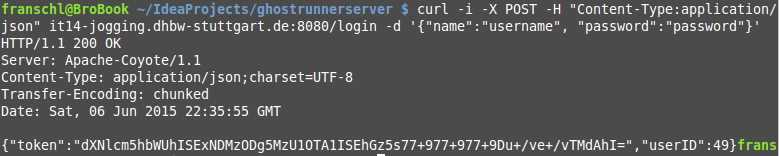
\includegraphics[width=\textwidth]{abb/curl_login}
\caption[Anmeldung]{Eine erfolgreiche Anmeldung mithilfe des Kommandozeilentools CURL}
\label{fig:Anmeldung}
\end{figure}
\paragraph{Authentifizierungstoken}
Das Authentifizierungstoken besteht, base64-dekodiert aus drei Teilen, getrennt durch jeweils drei Ausrufezeichen:
\begin{itemize}
\item Nutzername
\item Ablaufdatum des Tokens als UNIX-Zeitstempel (in Millisekunden)
\item geheimer Hash, der sich aus MD5-Hash des Nutzernamen, Salts und des Tokenablaufdatums zusammensetzt.
\end{itemize}

Dekodiert man z.B.  das erhaltene Token aus Abbildung~\ref{fig:Anmeldung} erhält man den folgenden String:
\begin{lstlisting}
username!!!1433889355905!!<eine Kette aus Sonderzeichen>
\end{lstlisting}
\paragraph{Nutzung des Sicherheitstokens}
Um sich mit dem Authentifizierungstoken am Server zu authentifizieren muss dieses bei jeder Anfrage des Klienten an den Server mitgeschickt werden.

Besonders zu Testzwecken empfiehlt es sich das Token per GET-Parameter in der URL mitzugeben. 

Eine Anfrage sieht dann z.B. so aus:
\begin{lstlisting}
it14-jogging.dhbw-stuttgart.de:8080/user/?token=<BeispielToken>
\end{lstlisting}

Eine weitere Option ist das Angeben des Tokens in der Kopzeile der Anfrage als das Attribut  ``authentication-token''.
\subsubsection{JSON - Serialisierung und Deserialisierung}\label{jackson}
Das Format der meisten Nachrichten zwischen Client und Server ist JSON.

Um den Aufwand zu minimieren und die Codeübersichtlichkeit zu maximieren wird dazu serverseitig das Tool Jackson in der Version 2.5.0 verwendet.

Es ist selbstständig in der Lage Klassen zu JSON-Objekten und Listen zu JSON-Arrays zu serialisieren und umgekehrt zu deserialisieren.

Die Einbindung erfolgt über Mavens pom.xml:
\lstset{language=xml}
\begin{lstlisting}[frame=htrbl, caption={Jacksons Abhängigkeiten in Maven}, breaklines=true]
<dependency>
	<groupId>com.fasterxml.jackson.core</groupId>
	<artifactId>jackson-core</artifactId>
	<version>2.5.0</version>
</dependency>

<dependency>
	<groupId>com.fasterxml.jackson.core</groupId>
	<artifactId>jackson-databind</artifactId>
	<version>2.5.0</version>
</dependency>

<dependency>
	<groupId>com.fasterxml.jackson.core</groupId>
	<artifactId>jackson-annotations</artifactId>
	<version>2.5.0</version>
</dependency>
\end{lstlisting}

In der mvc-dispatcher-servlet.xml wird die Bean eingebunden:
\lstset{language=xml}
\begin{lstlisting}[frame=htrbl, caption={Konfiguration von Jackson}, breaklines=true]
<bean id="jsonMessageConverter" class="org.springframework.http.converter.json.MappingJackson2HttpMessageConverter">
</bean>
\end{lstlisting}

Da Spring dank der ``component-scan''-Funktionalität von Spring MVC so konfiguriert ist, die Verzeichnisse automatisch nach Beans zu durchsuchen und diese einzubinden ist an dieser Stelle keine weitere Arbeit mehr nötig und Jackson tut seine Arbeit.

Wegen Hibernate kam es jedoch zu teils größeren Problemen mit Jackson. Diese liesen sich mittels einer weiteren Maven-Abhängigkeit eines speziell an Hibernate angepassten Jackson-Plugins und geringfügiger Änderungen im mvc-dispatcher-servlet.xml jedoch lösen:
\lstset{language=xml}
\begin{lstlisting}[frame=htrbl, caption={Einbindung von Jackson-datatype-hibernate4 in Maven}, breaklines=true]
<dependency>
	<groupId>com.fasterxml.jackson.datatype</groupId>
	<artifactId>jackson-datatype-hibernate4</artifactId>
	<version>2.4.0</version>
</dependency>
\end{lstlisting}
\lstset{language=xml}
\begin{lstlisting}[frame=htrbl, caption={Konfiguration von Jackson und Hibernate}, breaklines=true]
<mvc:annotation-driven>
        <mvc:message-converters>
            <bean class="org.springframework.http.converter.json.MappingJackson2HttpMessageConverter">
                <property name="objectMapper">
                    <bean class="com.springapp.HibernateAwareObjectMapper"/>
                </property>
            </bean>
        </mvc:message-converters>
    </mvc:annotation-driven>
\end{lstlisting}
\subsection{Android App}
Der folgende Abschnitt befasst sich mit einigen spannenden Elementen der Implementierung der Android App. Es werden aber bei weitem nicht alle implementierten Funktionen in diesem Kapitel angesprochen.
\subsubsection{Höhenberechnung}
Ziel des Höhenservice der App ist es, bei übergebenem Standort in Form von Längen- und Breitengrad eine der Position entsprechenden Höhe zurückzugeben.
\paragraph{Performance}
Durch die eigenständige Implementierung des Service haben wir den Vorteil, nicht mehr von Wartezeiten der Netzwerkkommunikation abhängig zu sein. Um diesen Vorteil ausnutzen zu können, ist es nötig, den Höhenservice möglichst performant zu gestalten. Das herunterladen und parsen der vergleichsweise großen Arcascii Dateien nimmt bei dem Prozess die meiste Zeit in anspruch, sollte also während des Laufs vermieden werden. Wir haben uns entschieden, alle Dateien vor Beginn des Laufs herunterzuladen, zu parsen und alle im Umkreis des Startstandorts des Nutzers liegenden Höhendaten in einem zweidimensionalen Array im Hauptspeicher zu sichern. Auf dieses kann während dem Lauf sehr schnell zugegriffen werden.

Zusätzlich ist es wichtig, die Dateirößen zu beschränken. Statt 5x5 Grad der original SRTM Files haben wir diese in kleiner Dateien der Größe 1x1 Grad aufgeteilt. Dies entspricht immer noch einem sehr großen Bereich von 110x110 Kilometern, die Dateigröße sinkt dadurch aber auf wenige Megabyte, was für einen einmaligen Download akzeptabel ist.
\paragraph{Parsen}
Nach Download der Dateien, die der Position des Nutzers entsprechen, müssen diese geparst werden. Zunächst muss hierbei die richtige Zeile für den entsprechenden Breitengrad gefunden werden. Vereinfacht zeigt das das folgende Code Snippet:
\lstset{language=java}
\begin{lstlisting}[frame=htrbl, caption={Finden der ersten benötigten Zeile}, breaklines=true]
while(row < headerlength + latitude - elevationArray.length) \{
	srtm.readLine();
\}
\end{lstlisting}
Sobald der Startpunkt gefunden wurde, wird unser zweidimensionales Höhenarray befüllt:
\lstset{language=java}
\begin{lstlisting}[frame=htrbl, caption={Füllen des Höhenarrays}, breaklines=true]
for(int i = 0; i < elevationArray.length; i++ \{
	String[] line = srtm.readLine().split(" ");
	for (int j = 0; j < arrayLength; j++) \{
                elevationArray[i][j] = Integer.parseInt(line[longitude + j]);
	\}
\}
\end{lstlisting}
Nicht beachtet wurde bei diesen Beispielen, dass Längen- und Breitengrad nicht direkt verwendet werden können, sondern zunächst in die entsprechenden Zeilen, bzw. Spalten der SRTM-Dateien umgerechnet werden müssen. Dieser Schritt hätte die Verständlichkeit des Beispielcodes unnötig erschwert.

Eine Herausforderung ergibt sich dann, wenn die Position des Nutzers sich in der Nähe von Dateigrenzen befindet. Dann ist es unter Umständen nötig, bis zu vier umliegende Dateien herunterzuladen, und das Array mit Teilen aller Dateien zu initialisieren.

Ist das Array initialisiert, kann ohne weiteres langwieriges Parsen direkt auf alle Höhendaten zugegriffen werden, die während des Laufs benötigt werden.
\subsubsection{Laufberechnung}
\paragraph{Ablauf}
Wird ein Lauf gestartet, starten wir dafür einen sogenannten \textit{Service}. Dieser erlaubt es, in Android Arbeiten im Hintergrund auszuführen, und deren Ergebnisse mit der Benutzeroberfläche zu kommunizieren. Die Höhenbestimmung ist ebenfalls als Service implementiert, der dem Laufservice bereitsteht.

Zu Beginn des Laufs wird zunächst das oben beschriebene Höhenarray initialisiert. Ist dies geschehen und kann eine Position gefunden werden, kann der Nutzer den Lauf starten.

Der Android \textit{FusedLocationService} erlaubt es, regelmäßige Positionsupdates anzufordern. Für jedes Update werden folgende Schritte durchlaufen:
\begin{itemize}
\item Position mit Längen- und Breitengrad ermitteln
\item Höhe ermitteln
\item Position im GPX tracken
\item Strecke seit letztem Update berechnen
\item Steigungsmultiplikator berechnen und Streckenabschnitt multiplizieren
\item Vergangene Zeit berechnen
\item Fortschritt in Prozent berechnen
\item Falls notwendig, Fortschritt der Geister in Prozent anhand der vergangenen Zeit berechnen
\item Position berechnen
\item Überprüfen, ob die Zielstrecke erreicht wurde und gegebenenfalls Lauf hochladen und beenden
\item Benutzeroberfläche aktualisieren
\end{itemize}
\paragraph{Steigungsausgleich}
Für den Steigungsausgleich wurde eine Methode  \textit{calcDistanceModifierFromSlope(Location[] locations)} erstellt, die einen Multiplikator als Fließkommazahl zurückgibt. Das Array \textit{locations[]} beinhaltet dabei die letzten zehn Positionen.

Die Implementierung der Methode sollte möglichst flexibel sein und gleichzeitig modular in den Lauf einfügbar sein, denn es kann erst durch ausgiebiges Testen und möglicherweise auch sportwissenschaftliche Analysen herausgefunden wie der Multiplikator genau aussehen muss. Deshalb findet die komplette Funktionalität des Höhenausgleichs an einer einzigen Stelle statt. Ein Rückgabewert von 1 entspricht keiner Streckenmodifikation, weshalb die App auch schon ohne vollständige Implementierung der Methode funktioniert.

Die primitivste Implementierung der Methode stellt ein einfaches, direktes Mapping der Steigung zwischen den letzten beiden Positionen dar. Es ist unwahrscheinlich, dass diese einen fairen Ausgleich darstellt, ist aber für anfängliche Tests gut geeignet.
\lstset{language=java}
\begin{lstlisting}[frame=htrbl, caption={Primitive Implementierung der Methode}, breaklines=true]
private double calcDistanceModifierFromSlope(Location[] locations) {
	double altitudeDelta = locations.getCurrentLocation().getAltitude() - locations.getLastLocation().getAltitude();
	double distance = locations.getLastLocation().distanceTo(locations.getCurrentLocation());
	double slope = altitudeDelta / distance;
	return slope;
}
\end{lstlisting}

Diese Methode kann optimiert werden, indem statt der Steigung ein modifizierter Wert zurückgegeben wird. Die Funktion dafür muss nicht unbedingt linear sein.

Außerdem können mehr als die letzten beiden Positionen zur Berechnung herangezogen werden. So kann der Multiplikatorbonus zusätzlich erhöht werden, wenn ein steiler Streckenabschnitt über längere Zeit gelaufen wird.


\section{Testen}\label{kapitel7}
%Logging, Testfälle

\section{Anwendungsbeispiel}\label{kapitel8}
%Eugen, Screenshots

%....

\section{Ausblick}\label{ausblick}
%global highscore
Die App befindet sich in einem recht frühen Stadium. Besonders auf die Kernfunktionalität - die des Laufes wurde viel wert gelegt. Dafür hätten wir uns gewünscht einige weitere Funktionalitäten umsetzen zu können bzw. vorhandene zu optimieren. 
\subsection{Sicherheit}
Wie im Abschnitt~\ref{sicherheit} beschrieben ist die Sicherheitskonfiguration der REST-API rudimentär. Hierbei prüft der Server lediglich auf die Existenz des Sicherheitstokens. Ist dieses gegeben kann jeder Nutzer andere u.A. Nutzer löschen oder deren Passwörter ändern.

\subsection{Globaler Vergleich}
Bisher ist die soziale Komponente der App komplett auf Gruppen beschränkt.

Um den Anreiz für das Laufen zu verstärken würde ein Vergleich mit allen anderen Nutzern sicher einen guten Weg darstellen. Dazu wäre es möglich eine globale Platzierung anzugeben, die den Läufer weiter motivieren könnte schnellere Zeiten zu laufen.

\subsection{Caching}
Die App ist so konzipiert dass alle Daten aus der REST-API beim Öffnen der jeweiligen Aktivität bzw. des jeweiligen Fragments geladen werden. 

Derartige Abfragen befinden sich zwar nicht im Hauptthread, jedoch wird der Inhalt erst dann angezeigt nachdem der Server antworten konnte.

Das führt dazu dass eine schlechte Internetverbindung die Navigation zu einer langwierigen Aufgabe werden lässt. Hier wäre es vorstellbar die Daten (z.B. Gruppen-, Nutzer- oder Laufinformationen) lokal zwischenzuspeichern, um die Datenverbindung zu schonen und eine flüssige Navigation zu garantieren.

\subsection{Fehlersicherheit}
Es bestehen eine Reihe an Möglichkeiten die App zum Absturz zu bringen. So kann während eines Lauf aufgrund des parallelen Zugriffs auf Google-Services die App nicht minimiert werden, ohne dass sie beim Maximieren eine Fehlermeldung anzeigt.

An weiteren Stellen kommt es unregelmäßig zu Fehlern, auf die programmatisch unzureichend reagiert wird.

Hier wäre ein recht kleiner Aufwand nötig um die Fehler in den Griff zu bekommen.

\subsection{Lockscreen-Widget}
Das Benutzen der App, besonders falls das Gerät mittels eines Passwortes o.Ä. entsperrt werden muss, kann sich als etwas mühsam gestalten.

Hier würde es sich anbieten ein Widget auf dem Lockscreen zu erstellen, das den aktuellen Fortschritt und relevante Informationen anzeigt. So ließe sich beim Laufen auf das regelmäßige Entsperren des Smartphones verzichten.

\subsection{Smartwatch-Konnektivität}
Als elegante Lösung um den aktuellen Fortschritt zu verfolgen würde die Ausgabe des Lauffortschritts auf einer Smartwatch dienen. Das kreisförmige Design beim Lauf ließe sich gut auf ein kleineres quadratisches Display übertragen.

Mittels einer Smartwatch ließe sich das Herausnehmen des Smartphones komplett vermeiden und würde so den Eingriff in den Lauf minimieren.

\section{Fazit}\label{fazit}
Das Projekt war ein voller Erfolg.

Innerhalb der App ist es möglich Läufe aufzuzeichnen, gegen ``Geister'' anderer anzutreten und sich innerhalb der Gruppen zu vergleichen. Zusätzlich sind weitere soziale Funktionalitäten wie die Einladung von Mitgliedern und Nichtmitgliedern implementiert.

Die REST-API tut ihre Arbeit und sorgt dafür dass ein kontrollierter Zugriff auf Ressourcen möglich ist.

Bei der Programmierung konnten die Mitglieder des Teams viel lernen.

Im Backend konnten sich die Mitglieder viel Wissen über die Programmierung der REST-API aneignen, besonders in Hinblick auf Sicherheit, Validierung und Web MVC in Spring, sowie auf Hibernate und MariaDB. 

Bei der Programmierung des Frontends konnten wir viel über Android-Entwicklung, insbesonders asynchrone Programmierung und Nutzeroberflächenentwicklung lernen.

%% Beispiel für Bild mit Fußnote
\begin{figure}[htb]
 \centering
 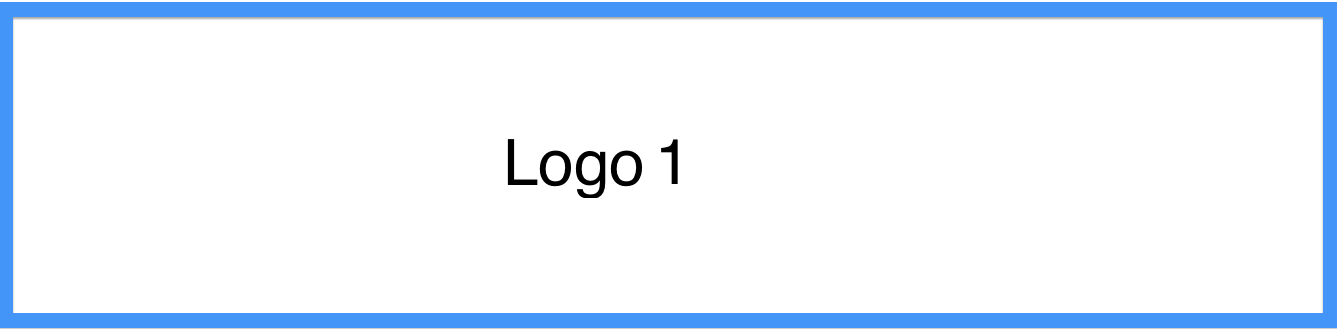
\includegraphics[width=0.4\textwidth,angle=45]{abb/logo1}
 \caption[Beispiel einer Bildbeschreibung]{Beispiel einer Bildbeschreibung\footnotemark}
\label{fig:beispiel1}
\end{figure}
\footnotetext{Bildquelle: Beispielquelle}

% Beispiel für Bildintegration
\begin{figure}[htb]
 \centering
 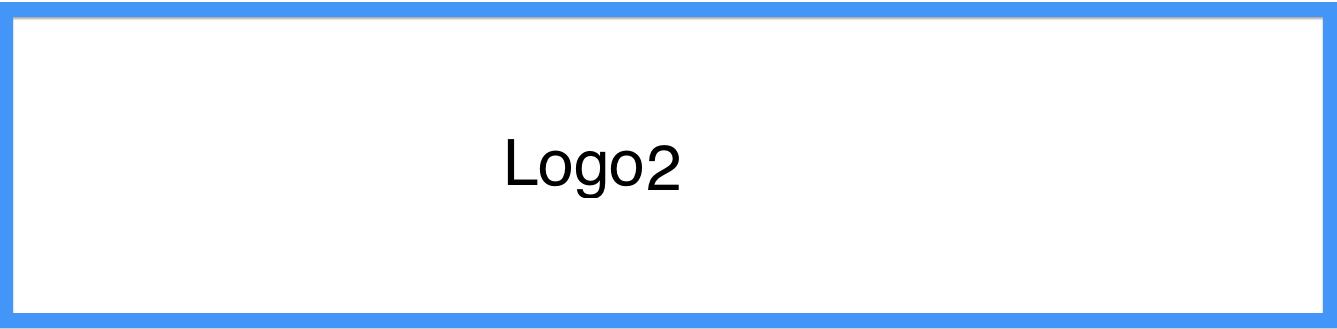
\includegraphics[width=0.3\textwidth,angle=0]{abb/logo2}
 \caption[Beschreibung]{Beschreibung}
\label{fig:Beschreibung}
\end{figure}

% Beispiel: Referenz auf Abbildung
Abbildung~\ref{fig:Beschreibung} [S.\pageref{fig:Beschreibung}]

% Beispiel: Tabelle 
\begin{center}
  \begin{tabular}{ | l | c | }
    \hline
    Überschrift 1 & Überschrift 2 \\ \hline \hline
    Info 1 & Info 2 \\ \hline
    Info 3 & Info 4 \\
    \hline
  \end{tabular}
\end{center}


% Beispiel für Quellcode Listings
\lstset{language=xml}
\begin{lstlisting}[frame=htrbl, caption={Die Datei {\tt data-config.xml} dient als Beispiel für XML Quellcode}, label={lst:dataconfigxml}]
<dataConfig>
  <dataSource type="JdbcDataSource" 
              driver="com.mysql.jdbc.Driver"
              url="jdbc:mysql://localhost/bms_db"
              user="root" 
              password=""/>
  <document>
    <entity name="id"
        query="select id, htmlBody, sentDate, sentFrom, subject, textBody
        from mail">
    <field column="id" name="id"/>
    <field column="htmlBody" name="text"/>
    <field column="sentDate" name="sentDate"/>
    <field column="sentFrom" name="sentFrom"/>
    <field column="subject"  name="subject"/>
    <field column="textBody" name="text"/>
    </entity>
  </document>
</dataConfig>
\end{lstlisting}

\lstset{language=java}
\begin{lstlisting}[frame=htrbl, caption={Das Listing zeigt Java Quellcode}, label={lst:result2}]
/* generate TagCloud */
Cloud cloud = new Cloud();
cloud.setMaxWeight(_maxSizeOfText);
cloud.setMinWeight(_minSizeOfText);
cloud.setTagCase(Case.LOWER);
	    
/* evaluate context and find additional stopwords */
String query = getContextQuery(_context);
List<String> contextStoplist = new ArrayList<String>();
contextStoplist = getStopwordsFromDB(query);
	    
/* append context stoplist */
while(contextStoplist != null && !contextStoplist.isEmpty())
  _stoplist.add(contextStoplist.remove(0));
	    
/* add cloud filters */
if (_stoplist != null) {
  DictionaryFilter df = new DictionaryFilter(_stoplist);
  cloud.addInputFilter(df);
}
/* remove empty tags */
NonNullFilter<Tag> nnf = new NonNullFilter<Tag>();
cloud.addInputFilter(nnf);

/* set minimum tag length */
MinLengthFilter mlf = new MinLengthFilter(_minTagLength);
cloud.addInputFilter(mlf);

/* add taglist to tagcloud */
cloud.addText(_taglist);

/* set number of shown tags */	    
cloud.setMaxTagsToDisplay(_tagsToDisplay);
\end{lstlisting}


% Beispiel für Formeln
Die Zuordnung aller möglichen Werte, welche eine Zufallsvariable annehmen kann nennt man \emph{Verteilungsfunktion} von $X$.

\begin{quotation}
Die Funktion F: $\mathbb{R} \rightarrow$ [0,1] mit $F(t) = P (X \le t)$ heißt Verteilungsfunktion von $X$.\footnote{Konen, vgl.~\cite{wk05}~[S.55]}
\end{quotation}

\begin{quotation}
Für eine stetige Zufallsvariable $X: \Omega \rightarrow \mathbb{R}$ heißt eine integrierbare, nichtnegative reelle Funktion $w: \mathbb{R} \rightarrow \mathbb{R}$ mit $F(x) = P(X \le x) = \int_{-\infty}^{x} w(t)dt$ die \emph{Dichte} oder \emph{Wahrscheinlichkeitsdichte} der Zufallsvariablen $X$.\footnote{Konen, vgl.~\cite{wk05}~[S.56]}
\end{quotation}


\onecolumn
% einfacher Zeilenabstand
\singlespacing
% Literaturliste soll im Inhaltsverzeichnis auftauchen
\newpage
\addcontentsline{toc}{section}{Literaturverzeichnis}
% Literaturverzeichnis anzeigen
\renewcommand\refname{Literaturverzeichnis}
\bibliography{Hauptdatei}

%% Index soll Stichwortverzeichnis heissen
% \newpage
% % Stichwortverzeichnis soll im Inhaltsverzeichnis auftauchen
% \addcontentsline{toc}{section}{Stichwortverzeichnis}
% \renewcommand{\indexname}{Stichwortverzeichnis}
% % Stichwortverzeichnis endgueltig anzeigen
% \printindex

\onehalfspacing
% evtl. Anhang
\newpage
\addcontentsline{toc}{section}{Anhang}
\fancyhead[L]{Anhang} %Kopfzeile links
\subsection*{Anhang}\label{anhang}


% Eidesstattliche Erklärung
\addcontentsline{toc}{section}{Eidesstattliche Erklärung}
\section*{Eidesstattliche Erklärung}
\thispagestyle{empty}

\begin{verbatim}

\end{verbatim}

\begin{LARGE}Eidesstattliche Erklärung zur <-Arbeit>\end{LARGE}
\begin{verbatim}


\end{verbatim}
Ich versichere, die von mir vorgelegte Arbeit selbstständig verfasst zu haben. Alle Stellen, die wörtlich oder sinngemäß aus veröffentlichten oder nicht veröffentlichten Arbeiten anderer entnommen sind, habe ich als entnommen kenntlich gemacht. Sämtliche Quellen und Hilfsmittel, die ich für die Arbeit benutzt habe, sind angegeben. Die Arbeit hat mit gleichem Inhalt bzw. in wesentlichen Teilen noch keiner anderen Prüfungsbehörde vorgelegen.



\begin{displaymath}
% use packages: array
\begin{array}{ll}
Unterschrift:~~~~~~~~~~~~~~~~~~~~~~~~~~~~~~~~~~~~~~~~~~
& Ort, Datum:~~~~~~~~~~~~~~~~~~~~~~~~~~~~~~~~~~~~~~~~~~
\end{array}
\end{displaymath}


\end{document}